\documentclass[10pt]{beamer}
%\documentclass[handout,10pt]{beamer}  % Remove pauses and disable commands like "onslide"
\usetheme[
%%% options passed to the outer theme
%    hidetitle,           % hide the (short) title in the sidebar
     hideauthor,          % hide the (short) author in the sidebar
%    hideinstitute,       % hide the (short) institute in the bottom of the sidebar
%    shownavsym,          % show the navigation symbols
%    width=2cm,           % width of the sidebar (default is 2 cm)
%    hideothersubsections,% hide all subsections but the subsections in the current section
%    hideallsubsections,  % hide all subsections
    left               % right of left position of sidebar (default is right)
%%% options passed to the color theme
%    lightheaderbg,       % use a light header background
]{AAUsidebar}

% If you want to change the colors of the various elements in the theme, edit and uncomment the following lines
% Change the bar and sidebar colors:
\definecolor{spartanBlue}{RGB}{0,85,162}
\definecolor{spartanYellow}{RGB}{229,168,35}
\definecolor{spartanGray}{RGB}{147,149,151}
\definecolor{darkGreen}{RGB}{34, 139, 34}

\setbeamercolor{frametitle}{use=structure,fg=white,bg=spartanBlue}
\setbeamercolor{title}{fg=frametitle.bg}

\setbeamercolor{header}{bg=spartanBlue}

\setbeamercolor{title in sidebar}{fg=frametitle.bg} % Headings on the side bar
\setbeamercolor{palette sidebar secondary}{fg=frametitle.bg} % Headings on the side bar
%\setbeamercolor{palette sidebar primary}{fg=frametitle.bg} % Slide titles (i.e., not slide sections)

\setbeamercolor{section in toc}{use=palette sidebar secondary,fg=palette sidebar secondary.fg} 
\setbeamercolor{subsection in toc}{use=normal text,fg=palette normal text.fg} 
\setbeamercolor{block title}{fg=spartanBlue} % Color of headings
\setbeamercolor{local structure}{fg=spartanBlue} % Color of enumerated items (e.g. lists, bullets, etc.)
\setbeamercolor{bibliography item}{use=local structure,fg=local structure.fg} % Color number of bibliography items
\setbeamercolor{bibliography entry author}{use=normal text,fg=normal text.fg} % Color bibliography entry.  Includes not just author but all fields


\usepackage{environ}
\usepackage{tikz}
\usepackage{listings} % Used for printing source code in papers
\usepackage{pgfplots} % Used to create graphs
\usepackage{makecell} % Used to create thick links in tables
\usepackage{algorithm} % Used for writing algorithms in a paper
\usepackage[noend]{algpseudocode} % Allows psuedocode keywords (e.g., "if", "while", "for", etc.) in algorithms.
\usepackage{xcolor, colortbl} % Used for coloring the cells of tables
\usepackage[utf8]{inputenc}
\usepackage[english]{babel}
\usepackage[T1]{fontenc}
% Or whatever. Note that the encoding and the font should match. If T1
% does not look nice, try deleting the line with the fontenc.
\usepackage{helvet}
\usepackage{makecell} % Used to create thick links in tables
\usepackage{multirow} % Allows merging rows or columns in a table

% Definitions for Custom Algorithmic Commands
\algdef{SE}[DOWHILE]{Do}{doWhile}{\algorithmicdo}[1]{\algorithmicwhile\ #1}
\algnewcommand\algorithmicforeach{\textbf{for each}}
\algdef{S}[FOR]{ForEach}[1]{\algorithmicforeach\ #1\ \algorithmicdo}
\algrenewcommand\alglinenumber[1]{\scriptsize #1:}

% colored hyperlinks
\newcommand{\chref}[2]{%
  \href{#1}{{\usebeamercolor[bg]{AAUsidebar}#2}}%
}

\DeclareMathOperator*{\argmax}{arg\,max} % The "*" means the limits go underneath "arg max"

% Transition slide
\newcommand{\transitionFrame}[1]{
{
  \begin{frame}[plain,noframenumbering]{}{} % the plain option removes the sidebar and header from the title page
	  \finalpage{{\Large \textbf{#1}}}
  \end{frame}}
}





\title[A Fully-Automated Solver for Multiple Square Jigsaw Puzzles Using Hierarchical Clustering]% optional, use only with long paper titles
{\textbf{A Fully-Automated Solver for Multiple Square Jigsaw Puzzles Using Hierarchical Clustering}}

\subtitle{}  % could also be a conference name

\date{October 27, 2016}

\author[Zayd Hammoudeh] % optional, use only with lots of authors
{
    Zayd Hammoudeh\\
    \href{mailto:hammoudeh@gmail.com}{{\tt hammoudeh@gmail.com}}
}
% - Give the names in the same order as they appear in the paper.
% - Use the \inst{?} command only if the authors have different
%   affiliation. See the beamer manual for an example

\institute[
%  {\includegraphics[scale=0.2]{aau_segl}}\\ %insert a company, department or university logo
    Dept.\ of Computer Science\\
    San Jos\'{e} State University\\
] % optional - is placed in the bottom of the sidebar on every slide
{% is placed on the title page
    Department of Computer Science\\
    San Jos\'{e} State University\\
  
  %there must be an empty line above this line - otherwise some unwanted space is added between the university and the country (I do not know why;( )
}


% specify a logo on the titlepage (you can specify additional logos an include them in 
% institute command below
\pgfdeclareimage[height=1.5cm]{titlepagelogo}{images/SJSU_Seal_Blue} % placed on the title page
\titlegraphic{% is placed on the bottom of the title page
  \pgfuseimage{titlepagelogo}
%  \hspace{1cm}\pgfuseimage{titlepagelogo2}
}


%%%%%%%%%%%%%%%%%%%%%%%%%%%%%%%%%%%%%%%%%%
%% Handles Slide Numbering For Appendix %%
%%%%%%%%%%%%%%%%%%%%%%%%%%%%%%%%%%%%%%%%%%
\newcommand{\backupbegin}{
   \newcounter{finalframe}
   \setcounter{finalframe}{\value{framenumber}}
}
\newcommand{\backupend}{
   \setcounter{framenumber}{\value{finalframe}}
}
%%%%%%%%%%%%%%%%%%%%%%%%%%%%%%%%%%%%%%%%%%


%%%%%%%%%%%%%%%%%%%%%%%%%%%%%%%%%%%%%%%%%%
%%   Scales tikz images to slide size   %%
%%%%%%%%%%%%%%%%%%%%%%%%%%%%%%%%%%%%%%%%%%
\makeatletter
\newsavebox{\measure@tikzpicture}
\NewEnviron{scaletikzpicturetowidth}[1]{%
  \def\tikz@width{#1}%
  \def\tikzscale{1}\begin{lrbox}{\measure@tikzpicture}%
  \BODY
  \end{lrbox}%
  \pgfmathparse{#1/\wd\measure@tikzpicture}%
  \edef\tikzscale{\pgfmathresult}%
  \BODY
}
\makeatother
%%%%%%%%%%%%%%%%%%%%%%%%%%%%%%%%%%%%%%%%%%


\begin{document}
% the titlepage
{
\begin{frame}[plain,noframenumbering]{}{} % the plain option removes the sidebar and header from the title page
	\titlepage
\end{frame}}
%%%%%%%%%%%%%%%%



%% Optional Table of Contents
%\begin{frame}{Agenda}{}
%	\tableofcontents
%\end{frame}
%%%%%%%%%%%%%%%%%



\section{Thesis Goals}
\begin{frame}{Introduction}{Thesis Goals}
  \onslide<1->{
    \textbf{Primary Goal}: Develop a solver that can assemble multiple jigsaw puzzles simultaneously, with performance that exceeds the state of the art.
    \vfill
  }
  \onslide<2->{
    \textbf{Additional Goals}:
    \vspace{0.4em}
    \begin{itemize}
      \setlength\itemsep{0.8em}
      \item Define the first metrics that quantify the quality of outputs from a multi-puzzle solver
      \item Design visualizations for viewing the errors (if any) in a solver output
    \end{itemize}    
  }
\end{frame}
%%%%%%%%%%%%%%%%



\section{Introduction}
\begin{frame}{Introduction}{Jigsaw Puzzles}
  \begin{itemize}
    \item First jigsaw puzzle introduced in the 1760s.  Modern jigsaw puzzles introduced in the 1930s.
    \vfill
    \item First computational jigsaw puzzle solver introduced in 1964
    \vfill
    \item Solving a jigsaw puzzle is NP-complete~\cite{altman1990, demaine2007}
    \vfill
    \item<2-> \textbf{Example Applications:} DNA fragment reassembly, shredded document reconstruction, speech descrambling, and image editing
    \begin{itemize}
        \item<3-> In most cases, the original, ``{\color{spartanBlue}\textbf{ground-truth}}'' image is unknown.
    \end{itemize}
  \end{itemize}
\end{frame}
%%%%%%%%%%%%%%%%


\begin{frame}{Introduction}{Jig Swap Puzzles}
    \textbf{Jig Swap Puzzles} -- Variant of the traditional jigsaw puzzle
    \begin{itemize}
        \item All pieces are equal-sized squares
        \item Substantially more difficult
    \end{itemize}
    \vfill
    % Delay the table on the slide
    \begin{tabular}{ 
      >{\centering\arraybackslash}m{0.45\textwidth} >{\centering\arraybackslash}m{0.45\textwidth} }
	    \onslide<2->{
	      \fbox{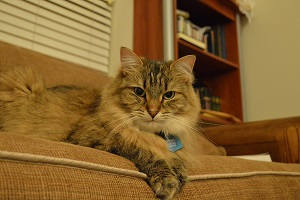
\includegraphics[width=0.365\textwidth]{./images/muffins_300x200.jpg}}
	    } & 
	    \onslide<3->{
	      \fbox{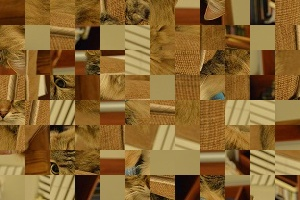
\includegraphics[width=0.365\textwidth]{./images/muffins_scrambled.jpg}}
	    }
	    \\ ~\\
	    \onslide<2->{
	      {\small Ground-Truth Image}
	    } & \onslide<3->{
	      {\small Randomized Jig Swap Puzzle}
	    }
	    \\ ~\\
  \end{tabular}
\end{frame}
%%%%%%%%%%%%%%%%



\begin{frame}{Introduction}{Jig Swap Puzzle Types}
\onslide<1->{There are three primary jig swap puzzle types as formalized by~\cite{gallagher2012}. In all cases, the ``ground-truth'' input is \textbf{unknown}.} 
    \vfill
    \begin{itemize}
        \item<2-> \textbf{Type~1}: Puzzle dimensions and piece rotation are known.  Only piece location is unknown.
        \vfill
        \item<3-> \textbf{Type~2}: All piece locations and rotations unknown.  Puzzle dimensions may be known.
        \vfill
        \item<4-> \textbf{Mixed-Bag}: Pieces come from multiple puzzles.
    \end{itemize}
    \vfill
    \onslide<5->{Mixed-Bag puzzles are the focus of this thesis.}
\end{frame}
%%%%%%%%%%%%%%%%



\subsection{Previous Work}

\begin{frame}{Previous Work}{Paikin \& Tal}
  \onslide<1->{
    {\color{spartanBlue}\textbf{Paikin \& Tal}}~\cite{paikin2015} -- Current State of the Art
    \begin{itemize}
      \setlength\itemsep{0.6em}
      \item Greedy, \textbf{kernel growing} solver
      \item Supports Type~1, Type~2, and Mixed-Bag puzzles
      \item Immune to missing pieces
    \end{itemize}    
  }
  \vfill
  \onslide<2->{
    {\color{spartanBlue}\textbf{Limitations}}:
    \begin{itemize}
      \setlength\itemsep{0.6em}
      \item \textbf{Poor Seed Selection}: All decisions are made at runtime using as few as 13 pieces
      \item \textbf{Externally Supplied Information}: The solver must be told the number of input puzzles
    \end{itemize}
  }
\end{frame}
%%%%%%%%%%%%%%%%



\section{Mixed-Bag Solver}
\transitionFrame{The Mixed-Bag Solver}



\begin{frame}{Mixed-Bag Solver}{Basic Structure}
  \begin{center}
    \fbox{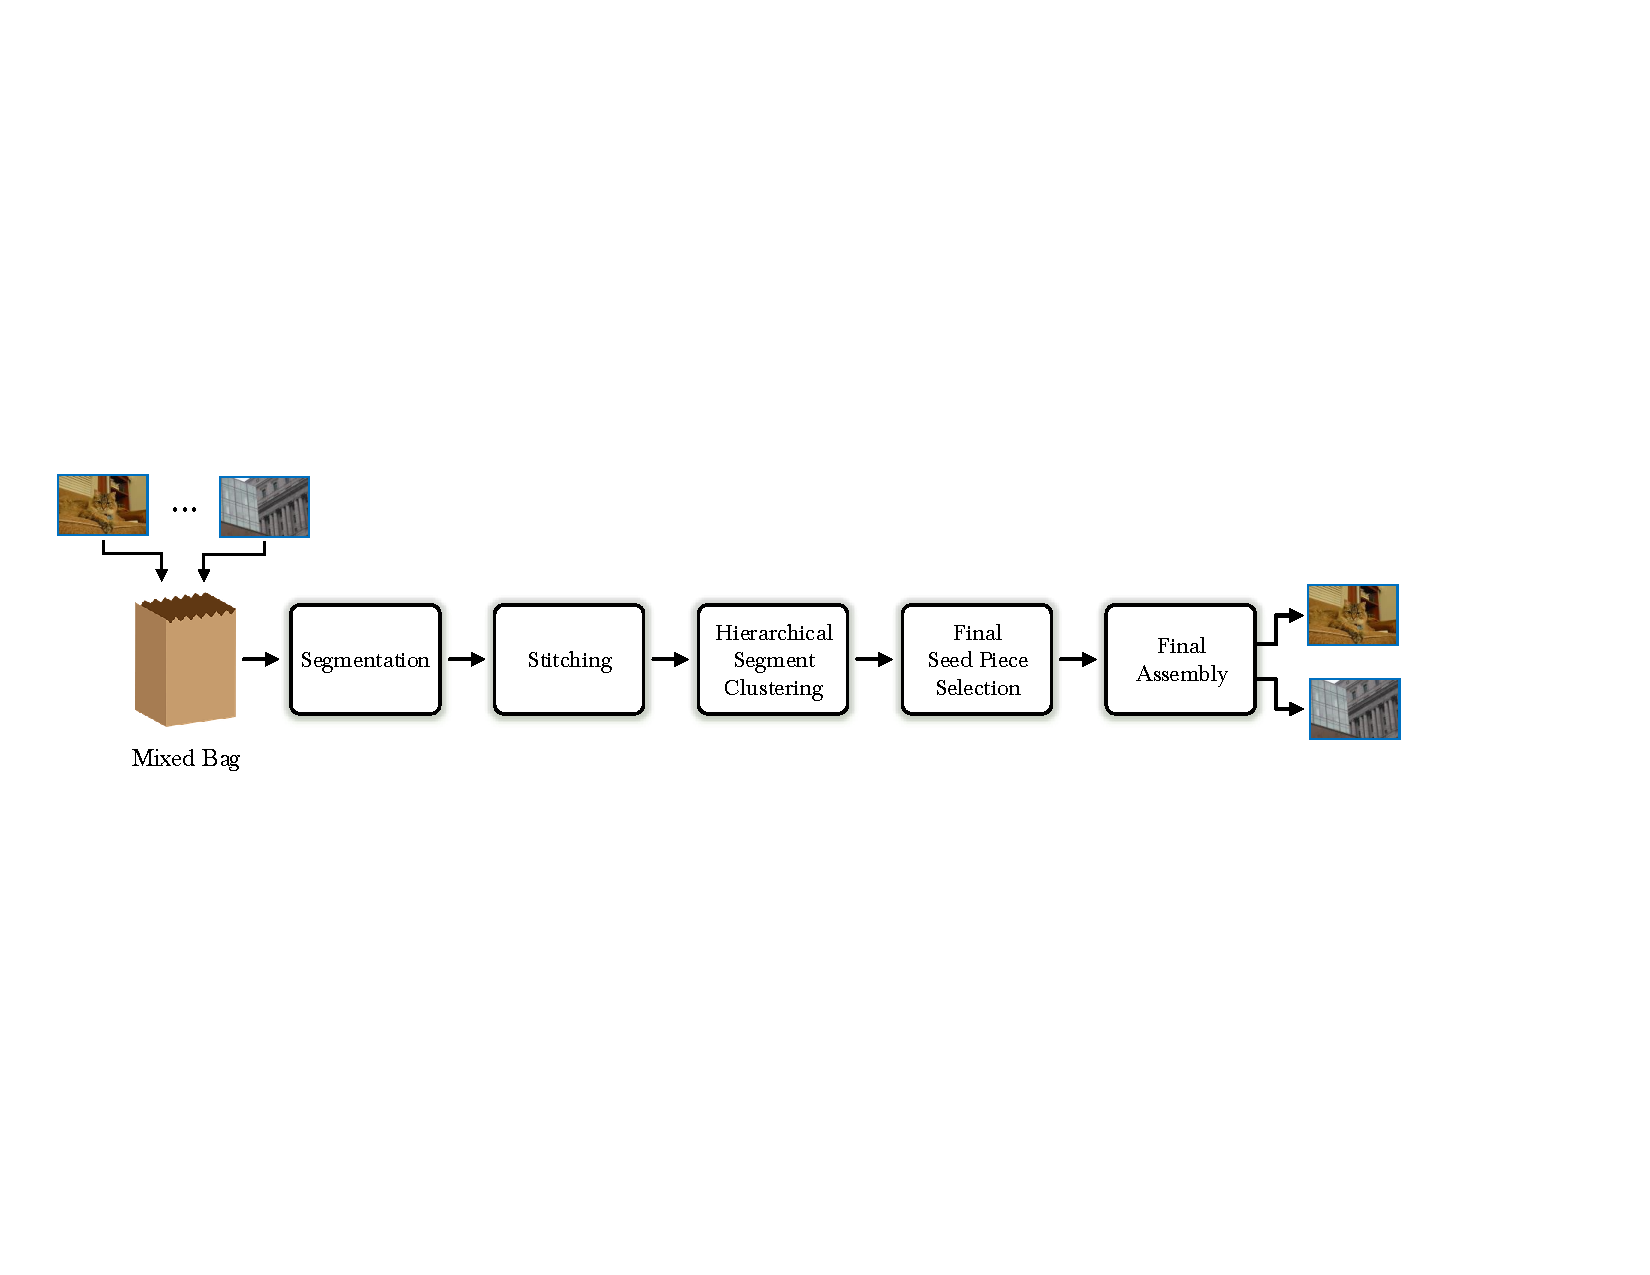
\includegraphics[width=0.95\textwidth]{./images/cropped_algorithm_structure_overview.pdf}}
    \vfill    
  \end{center}
\end{frame}
%%%%%%%%%%%%%%%%



\begin{frame}{Mixed-Bag Solver}{Foundations}
	\onslide<1->{\begin{block}{\textbf{Paikin~\& Tal's Algorithm}} 
	    \begin{itemize}
        \setlength\itemsep{.8em}
		    \item Begin each puzzle with a single piece
		    \item Place all pieces around the expanding kernel
	    \end{itemize}
	\end{block}}
	\vfill
	\onslide<2->{\begin{block}{\textbf{Alternate Jigsaw Puzzle Solving Strategy}}
    \begin{itemize}
      \setlength\itemsep{.8em}
			\item Correctly assemble small puzzle regions (i.e., segments)
			\item Iteratively merge smaller regions to form large ones	
			\onslide<3->{\item \textbf{Advantages of this Approach}: 
			\vspace{0.4em}
			\begin{itemize}
			    \setlength\itemsep{.8em}
			    \item Reduces the size of the problem
			    \item Provides structure to the unordered set of puzzle pieces.
			\end{itemize}}
    \end{itemize}
	\end{block}}
	\vfill
  \onslide<4->{The alternate strategy is the basis of the {\color{spartanBlue}\textbf{Mixed-Bag Solver}}}
\end{frame}



\begin{frame}{Mixed-Bag Solver}{Overview}
  \begin{itemize}
    \item The Mixed-Bag Solver is fully-automated.  It makes no assumptions concerning piece orientation, puzzle dimensions, or number of puzzles.
    \vspace{0.4em}
    \begin{itemize}
      \setlength\itemsep{0.8em}
      \item \textbf{Input}: A bag of puzzle pieces
      \item \textbf{Output}: One or more disjoint, solved puzzles.
    \end{itemize}
    \vfill    
    \item The Mixed-Bag Solver consists of five distinct stages:
	  \vspace{-0.4em}
  \end{itemize}
  \begin{center}
    \fbox{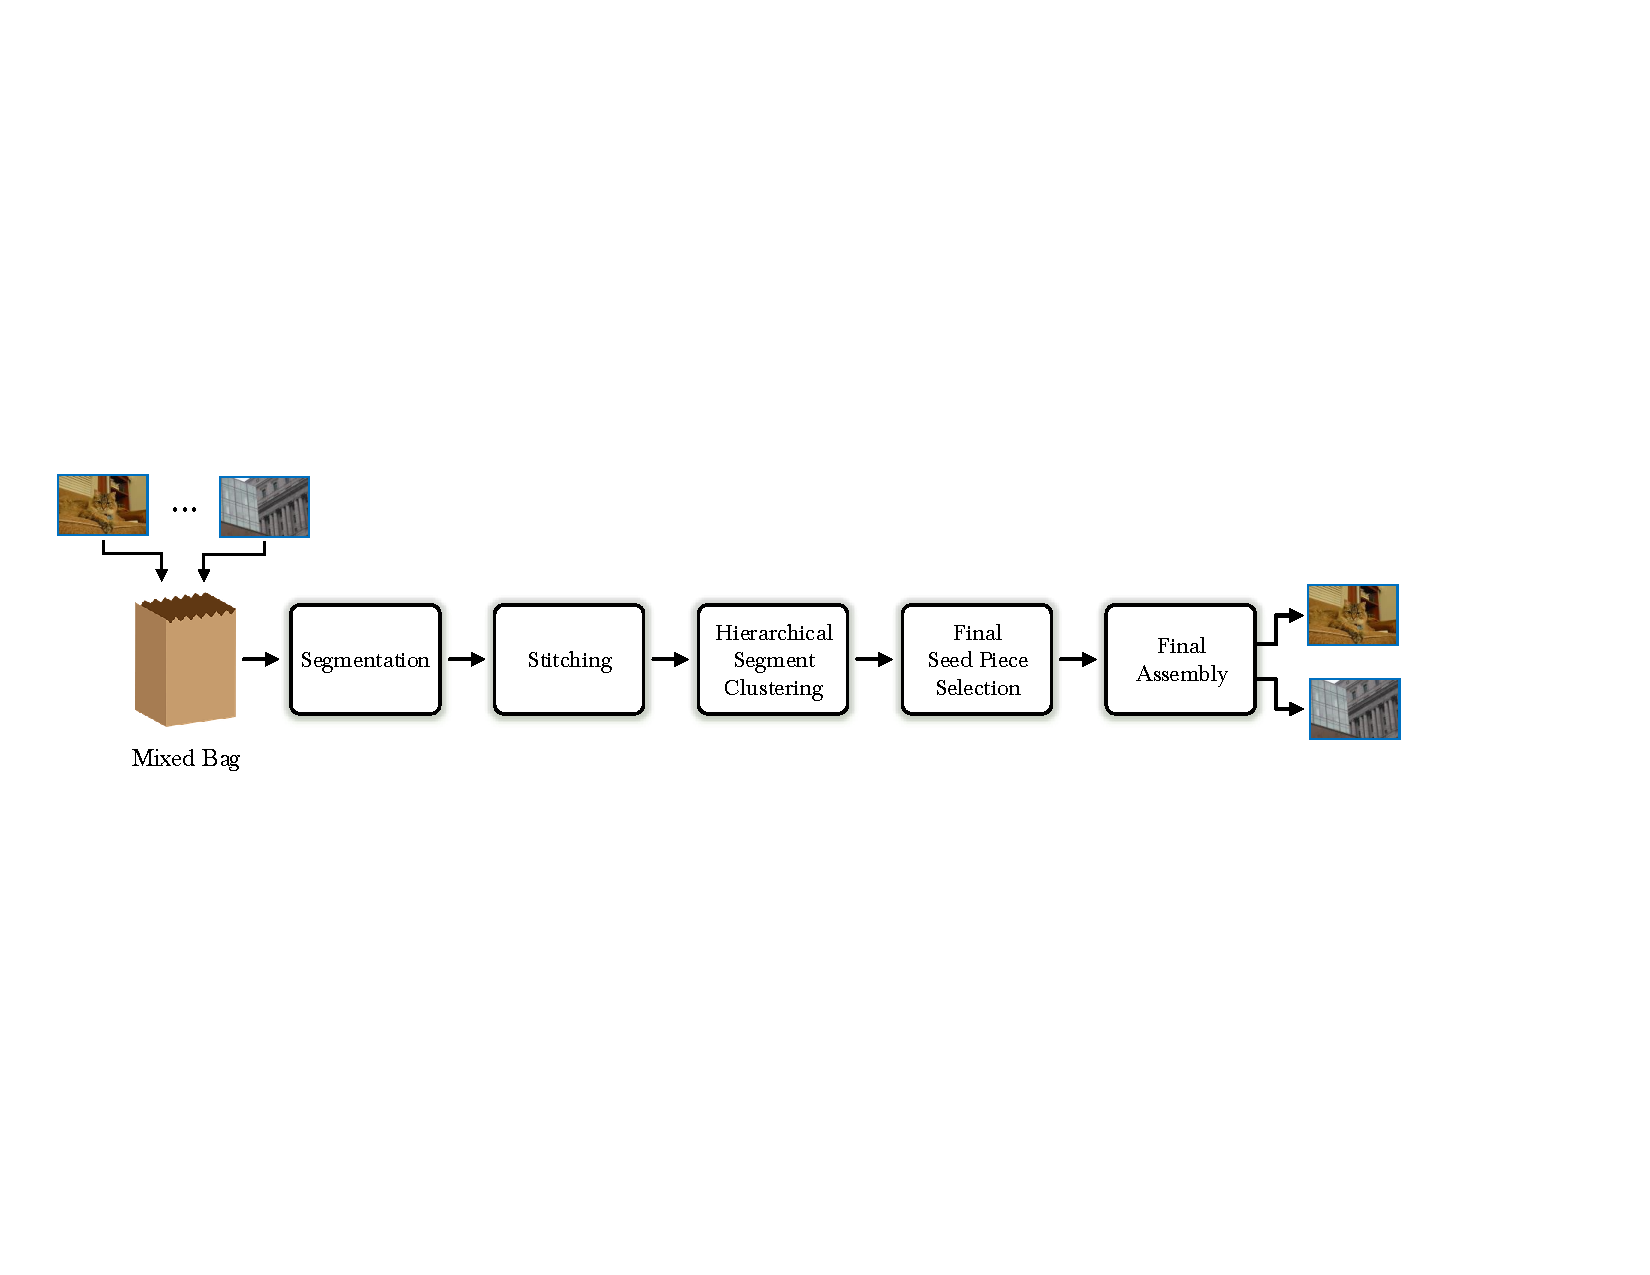
\includegraphics[width=0.96\textwidth]{./images/cropped_algorithm_structure_overview.pdf}}
    \vfill    
  \end{center}
\end{frame}
%%%%%%%%%%%%%%%%



\subsection{Assembler}
\begin{frame}{Assembler}{Mixed-Bag Solver Component}
  \begin{itemize}
    \onslide<1->{
	    \item \textbf{Role}: Place the individual pieces in the solved puzzle.
	    \vspace{0.4em}
	    \begin{itemize}
	      \setlength\itemsep{0.6em}
	      \item Mixed-Bag Solver is independent of the assembler used, giving the solver significant upgradability and flexibility.
	    \end{itemize}
	  }
    \vfill
    \onslide<2->{
	    \item \textbf{Assembler Used in this Thesis}: Paikin~\& Tal
	    \vspace{0.4em}
	    \begin{itemize}
	      \setlength\itemsep{0.6em}
	      \item Current state of the art
	      \item Allows for more direct comparison of performance
	      \item Natively supports Mixed-Bag puzzles
	    \end{itemize}
	    \vfill
	    \item \textbf{Implementation}: Assembler re-implemented as part of this thesis based off the description in~\cite{paikin2015}
	    \begin{itemize}
	      \item Written in Python and fully open source~\cite{githubThesisRepository}
	    \end{itemize}
	  }
  \end{itemize}
\end{frame}
%%%%%%%%%%%%%%%%




\subsection{Segmentation}
\begin{frame}{Segmentation}{Mixed-Bag Solver Stage \#1}
  \begin{itemize}
    \item \textbf{Segment}: Partial puzzle assembly where this is a high degree of confidence pieces are placed correctly.
    \vfill
    \item \textbf{Role of Segmentation}: Provide structure to the set of puzzle pieces by partitioning them into disjoint segments
    \begin{itemize}
      \vspace{0.4em}
      	\item \textbf{Input}: A bag of puzzle pieces
  		  \vspace{0.6em}
      \item \textbf{Output}: Set of saved segments
    \end{itemize}
	  \vfill
	  \item \textbf{Relationship between Puzzle Pieces and Segments}:
	  \vspace{0.4em}
	  \begin{itemize}
      \item Pieces from a single ground-truth input may be separated into multiple segments
  	  \vspace{0.6em}   
      \item A piece can be assigned to at most one segment   
    \end{itemize}
  \end{itemize}
\end{frame}



\begin{frame}{Segmentation}{Algorithm Overview}
  \begin{itemize}
    \item Iterative process consisting of one or more rounds  
    \vfill
    \item In each round, all pieces not yet assigned to a segment are assembled as if all are from the same input image
    \vfill
    \item Segments of sufficient size are saved to be used in future Mixed-Bag Solver stages
    \vfill
    \item Pieces in a saved segment are not placed in future rounds.
    \vfill
    \item Segmentation terminates if all pieces are assigned to a saved segment or when no segment is larger than the minimum allowed size
    \vfill
  \end{itemize}
\end{frame}
%%%%%%%%%%%%%%%%



\begin{frame}{Segmentation}{Composition of a Segment}
  \begin{itemize}
    \setlength\itemsep{0.8em}
    \item \textbf{Starting a Segment}: Each segment is created iteratively starting with a single seed piece
    \vfill
    \item \textbf{Definition of {\color{spartanBlue} Best Buddies}}: Any pair of pieces that are more similar to each other than they are to any other piece.
    \vfill 
    \item \textbf{Growing the Segment}: Add to the segment any piece that is a neighbor and best buddy of a segment member
    \vfill
    \item \textbf{Trimming the Segment}
    \vspace{0.4em}
    \begin{itemize}
    \setlength\itemsep{0.8em}
	    \item \textbf{Articulation Point}: Any piece whose removal disconnects other pieces from the segment seed.
	    \vspace{0.4em}
	    \begin{itemize}
	      \item All articulation pieces pieces are removed from the segment.  
	    \end{itemize}
	    \item After the removal of the articulation points, any pieces no longer connected to the seed are removed.
    \end{itemize}
  \end{itemize}
\end{frame}
%%%%%%%%%%%%%%%%




\begin{frame}{Segmentation}{Example -- Input Images}
  \vspace{-.4em}
  {\small 
  \begin{center}
	  \begin{tabular}{ 
	    >{\centering\arraybackslash}m{0.8\textwidth}}
		    \fbox{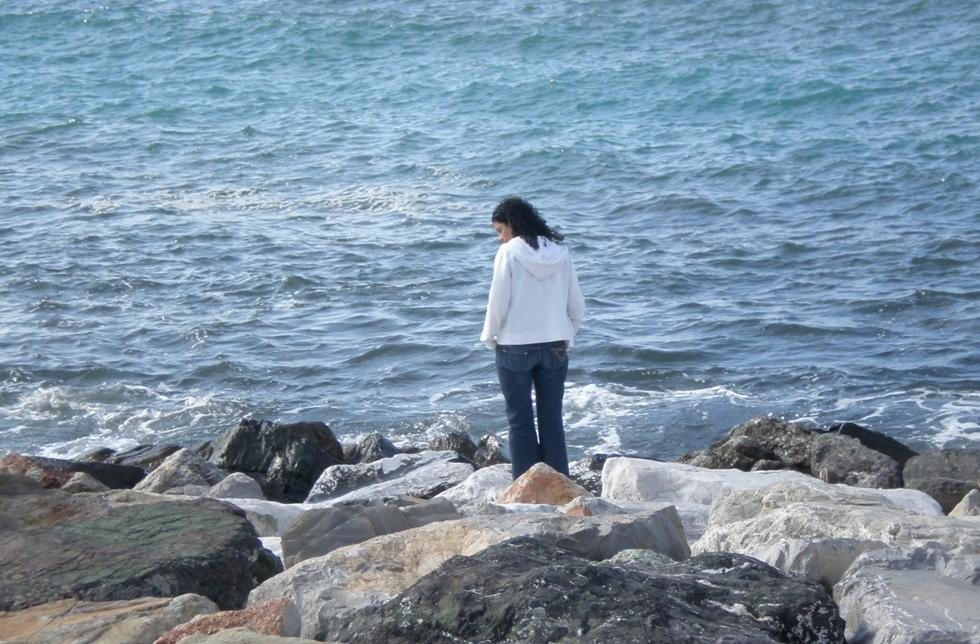
\includegraphics[scale=0.125]{./images/segmentation/pomeranz_805_8.jpg}}
		    \\[-0.2em]~\\[-0.2em]
		    Image~(a) \textendash { }805~Pieces~\cite{pomeranzBenchmarkImages}
	      \\~\\[-0.2em]
		    \fbox{\includegraphics[scale=0.125]{./images/segmentation/mcgill_540_20.jpg}}
	      \\[-0.2em]~\\[-0.2em]
		    Image~(b) \textendash { }540~Pieces~\cite{mcgillImageDatabase}
	  \end{tabular}
	\end{center}
	}
\end{frame}
%%%%%%%%%%%%%%%%


\begin{frame}{Segmentation}{Example -- First Segmentation Round Output Image}
  \begin{center}
	  \begin{tabular}{ 
	    >{ \centering\arraybackslash}m{0.9\textwidth} }
	    \fbox{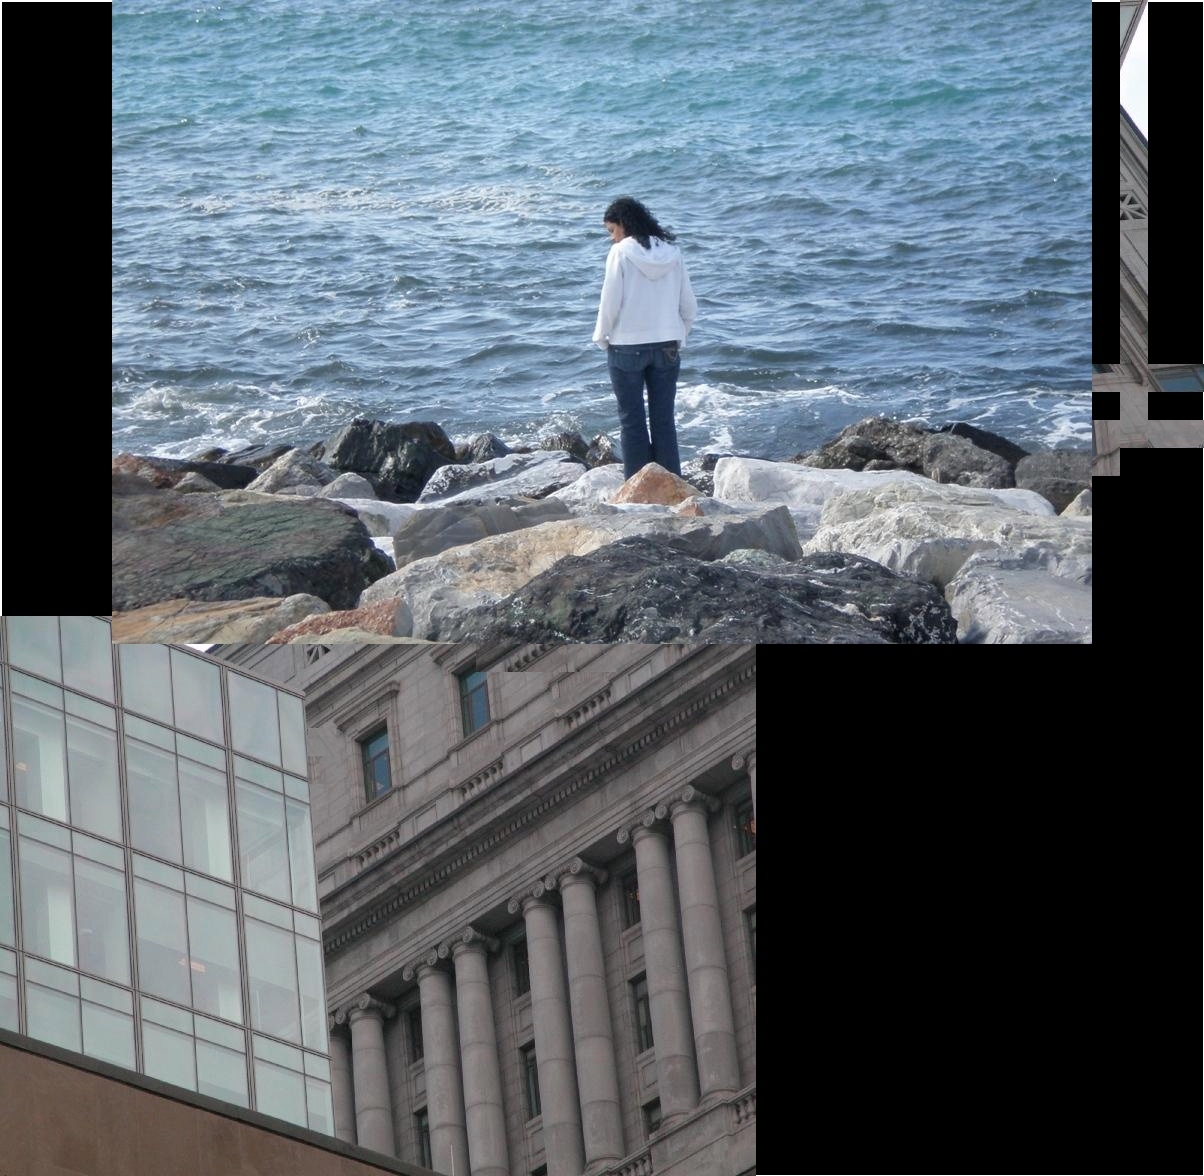
\includegraphics[scale=0.13]{./images/segmentation/assembler_single_puzzle_output.jpg}} 
	  \end{tabular}
  \end{center}
\end{frame}
%%%%%%%%%%%%%%%%



\begin{frame}{Segmentation}{Example -- Segmented Output Image}
  \begin{center}
	  \begin{tabular}{ 
	    >{ \centering\arraybackslash}m{0.9\textwidth} }
	    \fbox{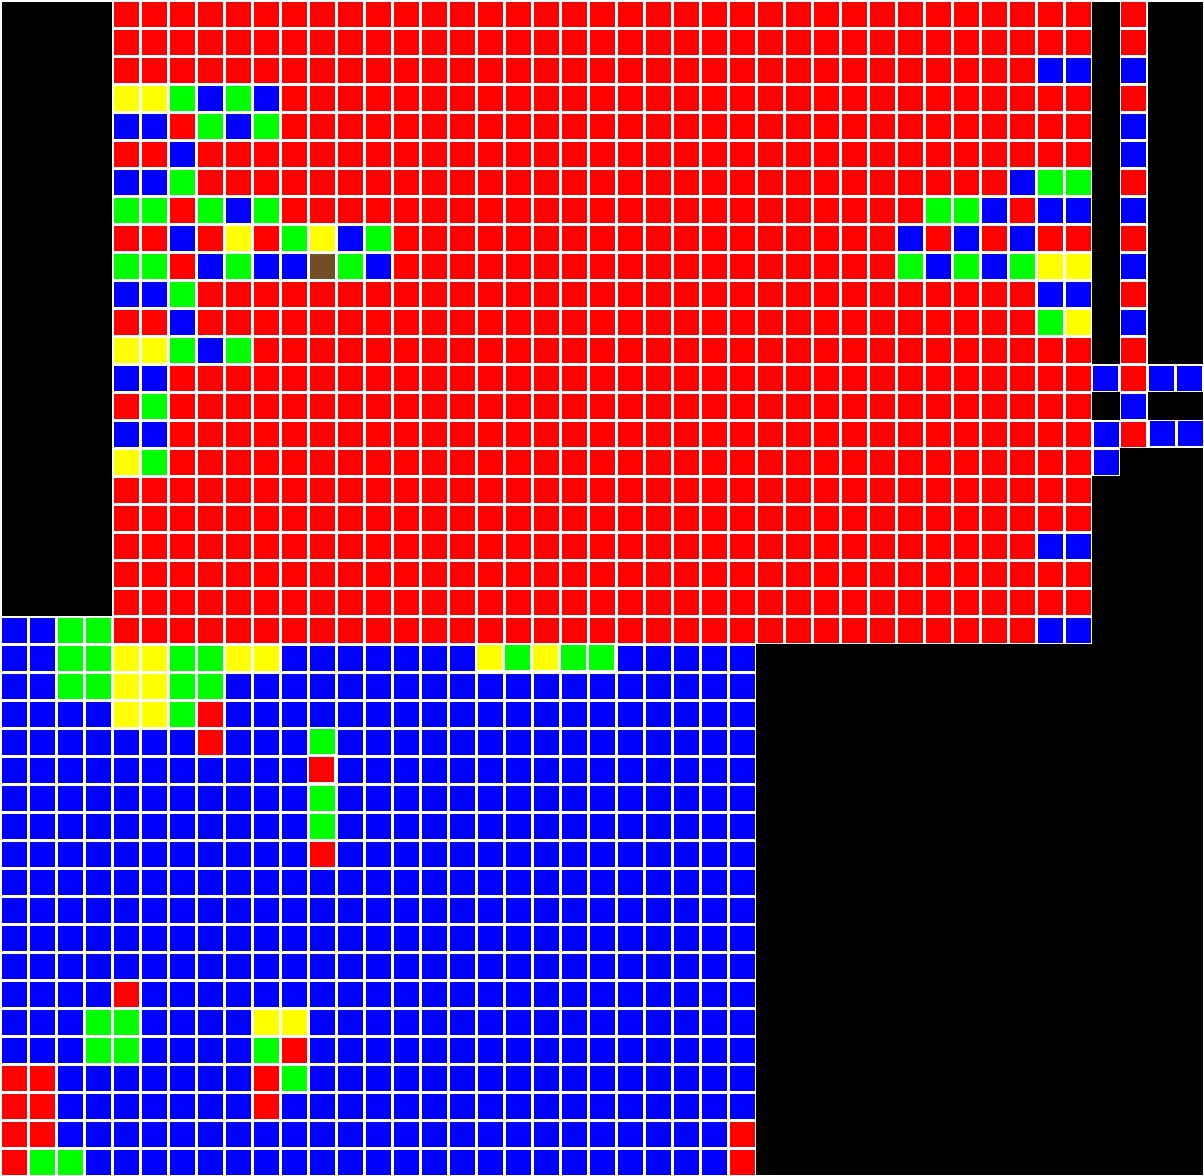
\includegraphics[scale=0.13]{./images/segmentation/segmented_single_puzzle_output.jpg}} 
	  \end{tabular}
  \end{center}
\end{frame}
%%%%%%%%%%%%%%%%



\subsection{Stitching}
\begin{frame}{Stitching}{Mixed-Bag Solver Stage \#2}
  \begin{itemize}
    \onslide<1->{
	    \item \textbf{Role of Stitching}: Quantify the extent that any pair of segments is related.
	    \begin{itemize}
	      \vspace{0.4em}
      	\item \textbf{Input}: All puzzle pieces and the set of saved segments
  		  \vspace{0.6em}
	      \item \textbf{Output}: Segment overlap matrix
	    \end{itemize}
	  }
	  \vfill
	  \onslide<2->{
	    \item \textbf{Theoretical Foundation}: If two segments are from the same ground-truth image, they would eventually {\color{spartanBlue}\textbf{overlap}} if one segment were to expand.
	    \vspace{0.4em}
	    \begin{itemize}
	      \setlength\itemsep{0.6em}
	      \item Segments should be allowed, but not forced, to expand in all directions.
	    \end{itemize}
	  }
  \end{itemize}
\end{frame}



\begin{frame}{Stitching}{Stitching Piece Location}
  \begin{itemize}
    \item \textbf{Mini-assembly} (\hspace{-0.1em}\textbf{$MA$}): Same as a standard assembly except only a fixed number of pieces are placed .
    \vfill    
    \item \textbf{Stitching Piece} (\textbf{$\zeta_x$}): A piece near the boundary of a segment that is used as the seed of a mini-assembly
    \vfill
    \item \textbf{Segment Overlap}: Maximum overlap between any mini-assembly for segment, $\Phi_i$ and another segment $\Phi_j$.
    \vfill
		\begin{center}  
		  \vspace{-2em}
			\begin{equation} \label{eq:segmentOverlap}
			  Overlap_{\Phi_i,\Phi_j} = \argmax_{\zeta_x \in \Phi_i} {\frac{|MA_{\zeta_x} \bigcap \Phi_j|}{\text{min}(|MA_{\zeta_x}|, |\Phi_j|)}}
			\end{equation}
			\vspace{-2em}
		\end{center}      
    \vfill
    \item \textbf{Asymmetry}: In most cases:
	  \begin{center}
	    \vspace{-2em}
	    \begin{equation}
	      Overlap_{\Phi_i,\Phi_j} \neq Overlap_{\Phi_j,\Phi_i}
	    \end{equation}
	  \end{center}  
	  \vspace{-1em}
  \end{itemize}
\end{frame}




\begin{frame}{Stitching}{Example -- Input Image}
  \begin{center}
    \fbox{\includegraphics[scale=0.25]{./images/stitching/mcgill_540_20.jpg}}
    \vfill    
  \end{center}
\end{frame}


\begin{frame}{Stitching}{Example -- Two Segment Images}
  \vspace{-.4em}
  {\small 
  \begin{center}
	  \begin{tabular}{>{\centering\arraybackslash}b{0.2\textwidth} >{\centering\arraybackslash}b{0.70\textwidth} }
	
		    \fbox{
\includegraphics[scale=0.23]{./images/stitching/stitching_image_segment_1.jpg}} 
		    & \fbox{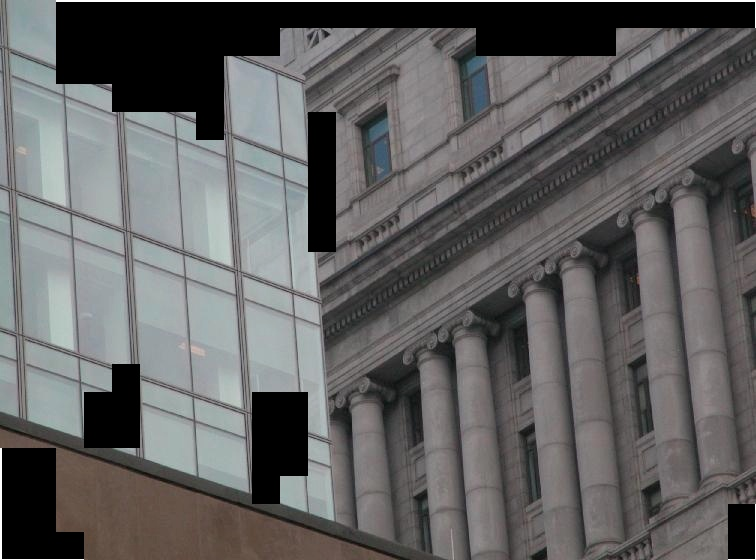
\includegraphics[scale=0.23]{./images/stitching/stitching_image_segment_2.jpg}}
		    \\~\\
		    \textbf{Segment \#1} & \textbf{Segment \#2}
	  \end{tabular}
	\end{center}
	}
\end{frame}


\begin{frame}{Stitching}{Example -- Stitching Piece Locations}
  \vspace{-.4em}
  {\small 
  \begin{center}
	  \begin{tabular}{>{\centering\arraybackslash}b{0.2\textwidth} >{\centering\arraybackslash}b{0.70\textwidth} }
	
		    \fbox{
\includegraphics[scale=0.23]{./images/stitching/stitching_pieces_segment_1.jpg}} 
		    & \fbox{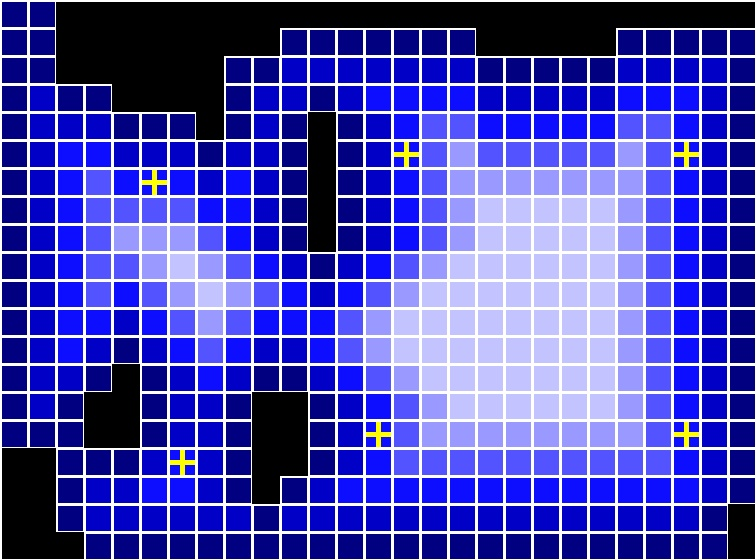
\includegraphics[scale=0.23]{./images/stitching/stitching_pieces_segment_2.jpg}}
		    \\~\\
		    \textbf{Segment \#1} & \textbf{Segment \#2}
	  \end{tabular}
	\end{center}
	}
\end{frame}



\begin{frame}{Stitching}{Example -- Stitching Piece Locations}
  \vspace{-.4em}
  {\small 
  \begin{center}
	  \begin{tabular}{>{\centering\arraybackslash}m{0.8\textwidth} }
	
		    \fbox{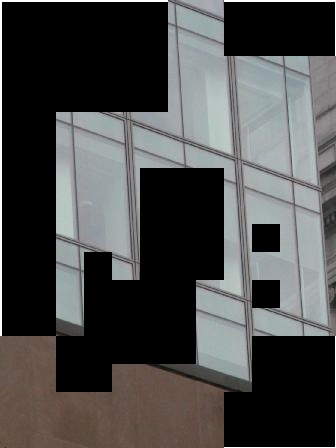
\includegraphics[scale=0.23]{./images/stitching/segment_1_stitching.jpg}} 
		    \\~\\
		    Stitching Result from Segment \#1
	  \end{tabular}
	\end{center}
	}
  \vfill
  \textbf{Segment Overlap:}
  \vspace{-2em}
  \begin{center}
    \begin{equation}
      Overlap_{\Phi_1,\Phi_2} = 0.83
    \end{equation}
  \end{center}  
\end{frame}


\subsection{Hierarchical Clustering}
\begin{frame}{Hierarchical Segment Clustering}{Mixed-Bag Solver Stage \#3}
  \begin{itemize}
    \item A single ground-truth image may be comprised of multiple segments.
    \vfill
    \item \textbf{Role of Hierarchical Clustering}: Merge all segments from the same input image into a single segment cluster.
    \begin{itemize}
      \vspace{0.4em}
      \item \textbf{Input}: All saved segments and the segment overlap matrix
  		\vspace{0.6em}
      \item \textbf{Output}: A set of {\color{spartanBlue}\textbf{segment clusters}}
    \end{itemize}
  \end{itemize}
\end{frame}



\begin{frame}{Hierarchical Segment Clustering}{Calculating the Initial Similarity Matrix}
  \begin{itemize}
    \item \textbf{Segment Overlap Matrix}: A hollow matrix quantifying the relationship between each pair of segments.
    \vspace{1em}
    \item \textbf{Hierarchical Clustering Similarity Matrix}: A diagonal matrix quantifying the similarity between segment pairs.
    \vspace{1em}
    \item \textbf{Quantifying Similarity}: Given $n$ segments, the similarity between segments $\Phi_i$ and $\Phi_j$ is:
  \end{itemize}
  \vspace{-1.5em}
  \begin{center}
    \begin{equation}
      \omega_{i,j} = \frac{Overlap_{\Phi_i, \Phi_j} + Overlap_{\Phi_j, \Phi_i}}{2} 
    \end{equation}
  \end{center}  
\end{frame}



\begin{frame}{Hierarchical Segment Clustering}{Merging Clusters}
  \begin{itemize}
    \item After two clusters are combined, the similarity between the merged cluster and all other clusters must be recalculated.
    \vfill
    \item \textbf{Single Link Clustering}: The similarity between any two clusters is equal to the maximum similarity between any two members in the clusters~\cite{tanIntroToDataMining}
    \vfill
    \item The Mixed-Bag Solver must use single link clustering as two clusters may only have two member segments that are adjacent.
  \end{itemize}
\end{frame}




\begin{frame}{Hierarchical Segment Clustering}{Example -- Single Linking}
  \begin{center}
    \fbox{\includegraphics[scale=0.25]{./images/stitching/mcgill_540_20.jpg}}
    \vfill    
  \end{center}
\end{frame}



\begin{frame}{Hierarchical Segment Clustering}{Example -- Single Linking}
  {\small 
  \begin{center}
  \setlength{\tabcolsep}{0pt}
	  \begin{tabular}{>{\centering\arraybackslash}b{0.175\textwidth} >{\centering\arraybackslash}b{0.24\textwidth}>{\centering\arraybackslash}b{0.20\textwidth}>{\centering\arraybackslash}b{0.185\textwidth}}
		    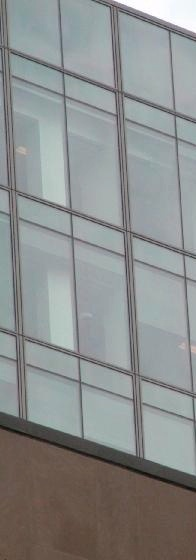
\includegraphics[scale=0.25]{./images/clustering/mcgill_20_segment_1.jpg}
		    & 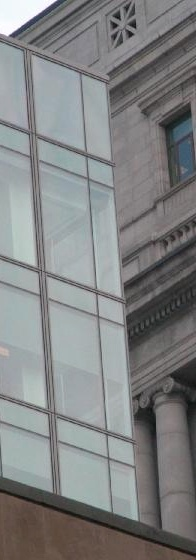
\includegraphics[scale=0.25]{./images/clustering/mcgill_20_segment_2.jpg}
		    & 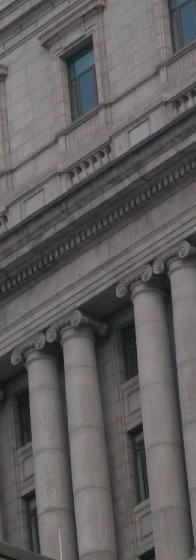
\includegraphics[scale=0.25]{./images/clustering/mcgill_20_segment_3.jpg}
		    & 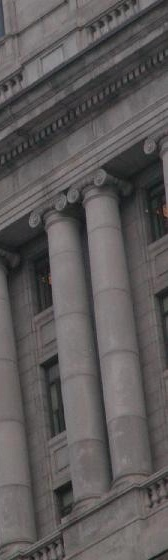
\includegraphics[scale=0.25]{./images/clustering/mcgill_20_segment_4.jpg}
		    \\~\\
		    Segment 1 & Segment 2 & Segment 3 & Segment 4
	  \end{tabular}
	\end{center}
	}
\end{frame}


\begin{frame}{Hierarchical Segment Clustering}{Example -- Single Linking}
  {\small 
  \begin{center}
  \setlength{\tabcolsep}{0pt}
	  \begin{tabular}{>{\centering\arraybackslash}b{0.45\textwidth}>{\centering\arraybackslash}b{0.20\textwidth}>{\centering\arraybackslash}b{0.185\textwidth}}
        \fbox{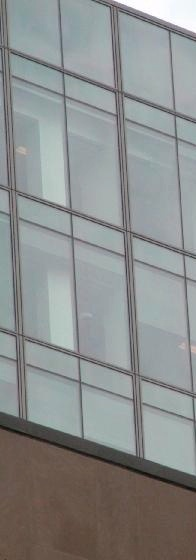
\includegraphics[scale=0.25]{./images/clustering/mcgill_20_segment_1.jpg}
		    \hspace{0.1in} 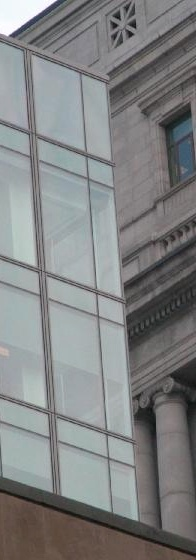
\includegraphics[scale=0.25]{./images/clustering/mcgill_20_segment_2.jpg}}
		    & 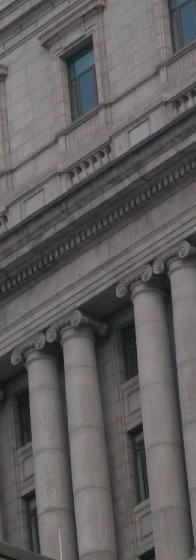
\includegraphics[scale=0.25]{./images/clustering/mcgill_20_segment_3.jpg}
		    & 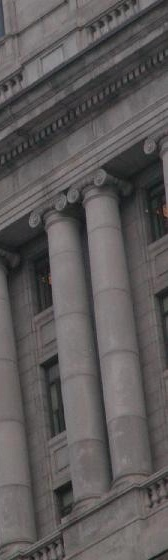
\includegraphics[scale=0.25]{./images/clustering/mcgill_20_segment_4.jpg}
		    \\~\\
		    Segment Cluster 1 & Segment 3 & Segment 4
	  \end{tabular}
	\end{center}
	}
\end{frame}



\begin{frame}{Hierarchical Segment Clustering}{Example -- Single Linking}
  {\small 
  \begin{center}
  \setlength{\tabcolsep}{0pt}
	  \begin{tabular}{>{\centering\arraybackslash}b{0.45\textwidth} >{\centering\arraybackslash}b{0.45\textwidth}}
		   \fbox{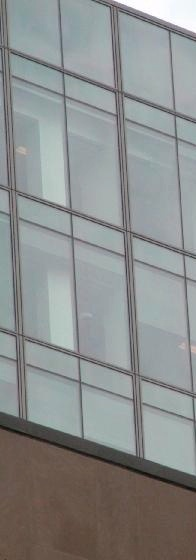
\includegraphics[scale=0.25]{./images/clustering/mcgill_20_segment_1.jpg}
		    \hspace{0.1in} 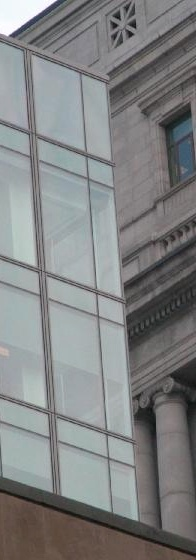
\includegraphics[scale=0.25]{./images/clustering/mcgill_20_segment_2.jpg}}
		    & \fbox{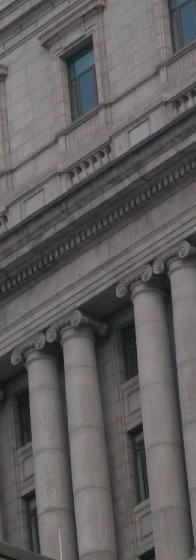
\includegraphics[scale=0.25]{./images/clustering/mcgill_20_segment_3.jpg}
		    \hspace{0.1in} 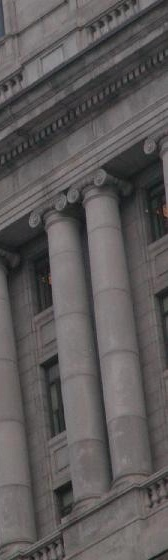
\includegraphics[scale=0.25]{./images/clustering/mcgill_20_segment_4.jpg}}
		    \\~\\
		    Segment Cluster 1 & Segment Cluster 2
	  \end{tabular}
	\end{center}
	}
\end{frame}



\begin{frame}{Hierarchical Segment Clustering}{Terminating Clustering}
  \begin{itemize}
  	\item The solver continues merging segment clusters until one of two criteria is satisfied:
	  \vspace{0.4em}
	  \begin{itemize}
	    \setlength\itemsep{0.8em}
	    \item Only a single segment cluster remains
	    \item Maximum similarity between any segment clusters is below a predefined threshold
	  \end{itemize} 
	  \vspace{1.5em}
	  \item All remaining segment clusters are passed to the next solver stage.
	\end{itemize}
\end{frame}





\subsection{Final Seed Piece Selection}
\begin{frame}{Final Seed Piece Selection}{Mixed-Bag Solver Stage \#4}
    \onslide<1->{    
      \begin{block}{\textbf{Mixed-Bag Solver}} 
        \vspace{0.4em}
        \begin{itemize}
          \item \textbf{Role of Final Seed Selection}: Determine the pieces that will be used as the seed for the final output puzzles.
          \vspace{0.4em}
          \begin{itemize}
            \item \textbf{Input}: Set of segment clusters
        	  \vspace{0.6em}
            \item \textbf{Output}: Final seed pieces
          \end{itemize}
          \vspace{0.6em}     
          \item A single seed piece is selected from each segment cluster
        \end{itemize}
      \end{block}
    }
    \onslide<2->{
      \begin{block}{\textbf{Paikin~\& Tal}}
        \vspace{0.4em}
        \begin{itemize}
          \item All puzzle seeds are selected greedily at run time, which often leads to poor decisions.
        \end{itemize}
      \end{block}
    }
\end{frame}
%%%%%%%%%%%%%%%%



\subsection{Final Assembly}
\begin{frame}{Final Assembly Stage}{Mixed-Bag Solver Stage \#5}
  \begin{itemize}

    \item \textbf{Role of Final Assembly}: Generate the solved puzzles that are output by the Mixed-Bag Solver.
	  \vspace{0.6em}
    \begin{itemize}
      \item \textbf{Input}: Set of puzzle pieces with the seeds marked
	    \vspace{0.6em}
      \item \textbf{Output}: Final solved puzzles
    \end{itemize}    
    \vspace{1.2em}
    \item All pieces are placed around the seeds selected in the previous stage.
    \vspace{1.2em}    
    \item Assembly proceeds in this stage normally without any custom modifications.
  \end{itemize}
\end{frame}
%%%%%%%%%%%%%%%%


\section{Quantifying Quality}
\transitionFrame{Quantifying Solver Quality}



\begin{frame}{Quantifying Solver Quality}{}
  \begin{itemize}
    \onslide<1->{
      \item Jigsaw puzzle solvers are not able to always correctly reconstruct the input puzzle(s)
      \vspace{0.4em}
      \begin{itemize}
        \item Metrics compare the quality of solver outputs
      \end{itemize}
      \vfill
      \item \textbf{Two Most Common Quality Metrics}:
      \vspace{0.4em}
      \begin{itemize}
        \setlength\itemsep{0.8em}
        \item Direct Accuracy
        \item Neighbor Accuracy
      \end{itemize}
    }
    \vfill 
    \onslide<2->{
      \item \textbf{Disadvantages of Current Metrics}: Neither account for:
      \vspace{0.4em}
      \begin{itemize}
        \setlength\itemsep{0.8em}
        \item Pieces misplaced in different puzzles
        \item Extra pieces from other puzzles
      \end{itemize}
      \vfill
      \item \textbf{Goal}: Define new quality metrics for Mixed-Bag puzzles
    }
  \end{itemize}
\end{frame}
%%%%%%%%%%%%%%%%




\subsection{Direct Accuracy}
\begin{frame}{Quantifying Solver Quality}{Standard and Enhanced Direct Accuracy}
  \onslide<1->{
    \begin{itemize}
      \item \textbf{Standard Direct Accuracy}: Fraction of pieces, $c$ placed in the same location in both the ground-truth and solved image versus the total number of pieces, $n$
    \end{itemize}
    \vfill
    \begin{equation}\label{eq:directAccuracy}
      DA = \frac{c}{n}
    \end{equation}
    \vspace{-0.8em}
  }
  \vfill
  \onslide<2->{
    \begin{itemize}
      \item \textbf{Enhanced Direct Accuracy Score (EDAS)}: Modified direct accuracy that accounts for missing and extra pieces.
    \end{itemize}
    \vfill
    \begin{equation}\label{eq:enhancedDirectAccuracyScore}
      EDAS_{P_i} = \argmax_{S_j \in S}\frac{c_{i,j}}{n_i + \sum_{k \ne i}(m_{k,j})}
    \end{equation}
    \vspace{-0.8em}
  }
  \vfill
  \onslide<3->{
    \begin{itemize}
      \item \textbf{Direct Accuracy Range}: 0 to 1
      \vfill
      \item \textbf{Perfectly Reconstructed Image}: All pieces are placed in their original location ($DA = EDAS = 1$)
    \end{itemize}
  }
\end{frame}
%%%%%%%%%%%%%%%%



\begin{frame}{Direct Accuracy}{Example -- Effect of Shifts}
  \onslide<1->{
    \textbf{Problem}: Direct accuracy is highly vulnerable to shifts, in particular when puzzle dimensions are not fixed
    \vfill
  }
  \begin{figure}
    \centering
    \begin{tabular}{ 
      >{\centering\arraybackslash}m{0.44\textwidth} >{\centering\arraybackslash}m{0.47\textwidth} }
	    \onslide<2->{
	      \fbox{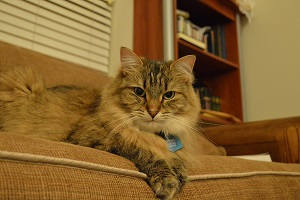
\includegraphics[width=0.41\textwidth]{./images/muffins_300x200.jpg}}
	    } &
	    \onslide<3->{
	      \fbox{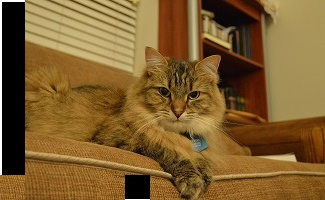
\includegraphics[width=0.44\textwidth]{./images/muffins_300x200_type1.jpg}}
	    }
	    \\ ~\\
	    \onslide<2->{
	      Ground-Truth Image
	    } & 
	    \onslide<3->{
	      Solver Output
	    } 
	    \\ ~\\
  \end{tabular}
  \label{fig:directAccuracyOnePieceEffect}
  \end{figure}
  \vspace{-2em}
  \vfill  
  \onslide<4->{
    \center{\textbf{Conclusion}: Direct accuracy can be overly punitive.}
  }
\end{frame}
%%%%%%%%%%%%%%%%



\begin{frame}{Direct Accuracy}{Shiftable Enhanced Direct Accuracy Score (SEDAS)}
  \begin{itemize}
    \item \textbf{Solution}: Allow the reference point for direct accuracy to {\color{spartanBlue}\textbf{shift beyond the upper left corner}} of the image
    \vfill
    \item \textbf{Shiftable Enhanced Direct Accuracy Score (SEDAS)}: Select the reference point, $l$, within radius $d_{min}$ of the upper left corner of the solved puzzle
    \begin{itemize}
      \vspace{0.6em}
      \item $d_{min}$ -- Manhattan distance between the upper left corner of the solved image and the nearest puzzle piece
    \end{itemize}
    \vfill
    \item \textbf{Formal Definition of SEDAS}:
  \end{itemize}
  \vfill  
  \begin{equation} \label{eq:shiftableEnhancedDirectAccuracyScore}
    SEDAS_{P_i} = \argmax_{l \in L} \bigg( \argmax_{S_j \in S}\frac{c_{i,j,l}}{n_i + \sum_{k \ne i}(m_{k,j})} \bigg)
  \end{equation}
  \vspace{-1em}
  \vfill
  \begin{itemize}
    \item \textbf{SEDAS Range}: 0 to 1
  \end{itemize}
\end{frame}
%%%%%%%%%%%%%%%%



\begin{frame}{Direct Accuracy}{Example -- Shiftable Reference Point}
  \begin{figure}
    \centering
    \begin{tabular}{ 
      >{\centering\arraybackslash}m{0.44\textwidth} >{\centering\arraybackslash}m{0.44\textwidth} }
	    \onslide<1->{
	      \fbox{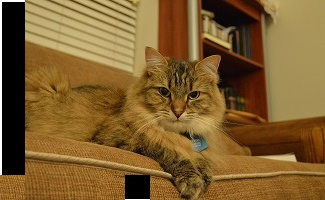
\includegraphics[width=0.40\textwidth]{./images/muffins_300x200_type1.jpg}}
	    } &
	    \only<2>{\fbox{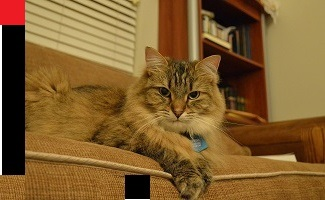
\includegraphics[width=0.40\textwidth]{./images/muffins_300x200_type1_EDAS.jpg}}}\only<3>{\fbox{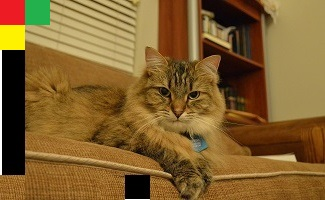
\includegraphics[width=0.40\textwidth]{./images/muffins_300x200_type1_SEDAS.jpg}}}
	    \\ ~\\
	    \onslide<1->{
	      {\footnotesize Solver Output}
	    } & 
	    \only<2>{\footnotesize Direct Accuracy Reference Point}\only<3>{\footnotesize SEDAS Reference Points} 
	    \\ ~\\
  \end{tabular}
  \end{figure}
\end{frame}
%%%%%%%%%%%%%%%%





\subsection{Neighbor Accuracy}
\begin{frame}{Quantifying Solver Quality}{Standard and Enhanced Neighbor Accuracy}
  \onslide<2->{
    \begin{itemize}
      \item \textbf{Standard Neighbor Accuracy}: Ratio of puzzle piece sides adjacent in both the original and solved images, $a$, versus the total number of sides, $n \cdot q$
    \end{itemize}
    \vfill
    \begin{equation}\label{eq:neighborAccuracy}
      NA = \frac{a}{n \cdot q}
    \end{equation}
    \vspace{-1em}
    \vfill
  }
  \onslide<3->{
    \begin{itemize}
      \item \textbf{Enhanced Neighbor Accuracy Score (ENAS)}: Modified neighbor accuracy that accounts for missing and extra pieces.
    \end{itemize}
    \vfill
    \begin{equation}\label{eq:enhancedNeighborAccuracyScore}
      ENAS_{P_i} = \argmax_{S_j \in S}\frac{a_{i,j}}{q (n_i + \sum_{k \ne i}(m_{k,j})}
    \end{equation}
    \vspace{-0.5em}
  }
  \onslide<4->{
    \vfill  
    \begin{itemize}
      \item \textbf{Neighbor Accuracy Range}: 0 to 1
      \vfill
      \item \textbf{Advantage of Neighbor Accuracy}: Less vulnerable to shifts than direct accuracy
    \end{itemize}
  }
\end{frame}
%%%%%%%%%%%%%%%%


\begin{frame}{Quantifying Solver Quality}{Visualizing Accuracy}
  \begin{itemize}
    \item The thesis includes visualization standards for direct and neighbor accuracy.
    \vfill
    \item They are not reviewed here due to limited time.
  \end{itemize}
\end{frame}
%%%%%%%%%%%%%%%%



\section{Experimental Results}
\transitionFrame{Experimental Results}



\begin{frame}{Experimental Results}{} 
  \begin{itemize}
    \onslide<2->{
      \item Paikin~\& Tal's algorithm is the current state of the art and was used as the reference for performance comparison
    }
    \vfill
    \onslide<3->{
      \item \textbf{Standard Test Conditions}:
        \begin{itemize}
          \setlength\itemsep{.3em}
          \item \textbf{Puzzle Type}: 2
          \item \textbf{Dimensions Fixed}: No
          \item \textbf{Piece Width}: 28~pixels
          \item \textbf{Benchmark}: Twenty 805~piece images~\cite{pomeranzBenchmarkImages}
      \end{itemize}
    }
  \end{itemize}
  \vfill
  \onslide<4->{
    \vspace{-0.6em}
    \begin{itemize}
      \item \textbf{Number of Ground-Truth Inputs}: 1 to 5
    \end{itemize}
    \vspace{-0.8em}
    \begin{center}
	    {\setlength\extrarowheight{2pt}      
	      \begin{tabular}{ |c||c|c|c|c|c| } 
	        \Xhline{1pt}
	        \# Puzzles    & 1 &  2 &  3 & 4 & 5 \\ 
	        \hline \hline
	        \# Iterations & 20 & 55 & 25 & 8 & 5 \\ 
	        \Xhline{1pt}
	      \end{tabular}
      }
    \end{center}
  }
  \vspace{-0.8em}    
  \vfill
  \onslide<5->{
    \begin{itemize}
      \item \textbf{Test Condition Variation}: Only Paikin~\& Tal's algorithm was provided the number of input puzzles.
    \end{itemize}
  }
\end{frame}
%%%%%%%%%%%%%%%%


\begin{frame}{Experimental Results}{Determining Input Puzzle Count}
  \begin{itemize}
    \onslide<1->{
      \item \textbf{Goal}: Measure the Mixed-Bag Solver's accuracy determining the number of input puzzles
      \vspace{0.4em}
      \begin{itemize}
        \item \textbf{Importance} -- The Mixed-Bag Solver must estimate this accurately to provide meaningful outputs.
      \end{itemize}
    }
    \onslide<2->{
      \vfill
      \item \textbf{Single Puzzle Accuracy} -- Represents the solver's performance ceiling
      \vfill
      \item \textbf{Multiple Puzzle Accuracy} -- A more general estimate of the solver's performance
    }
  \end{itemize}
\end{frame}
%%%%%%%%%%%%%%%%



\subsection{Input Puzzle Count}
\begin{frame}{Determining Input Puzzle Count}{Single Input Puzzle Results}
  \begin{itemize}
    \onslide<1->{
      \item \textbf{Summary}: 17~out of the 20 images were correctly identified as a single ground-truth input
      \vfill
      \item \textbf{Misclassified Images}: 3 out of the 20 images misclassified as if they were two images.
         \begin{itemize}
           \setlength\itemsep{.8em}
           \item All three images have large areas with little variation (e.g., a blue sky, smooth water)
           \item The solver's poor performance on these puzzles is due to the assembler as noted in~\cite{paikin2015}
         \end{itemize}
    }
    \vfill
    \onslide<2->{
      \item \textbf{Note}:~85\% (17/20) represents the accuracy ceiling when solving multiple puzzles.
    }
  \end{itemize}
\end{frame}
%%%%%%%%%%%%%%%%



\begin{frame}{Determining Input Puzzle Count}{Visual Comparison of a Misclassified Image}
  \begin{tabular}{ >{\centering\arraybackslash}m{0.44\textwidth} >{\centering\arraybackslash}m{0.44\textwidth} }
	  \fbox{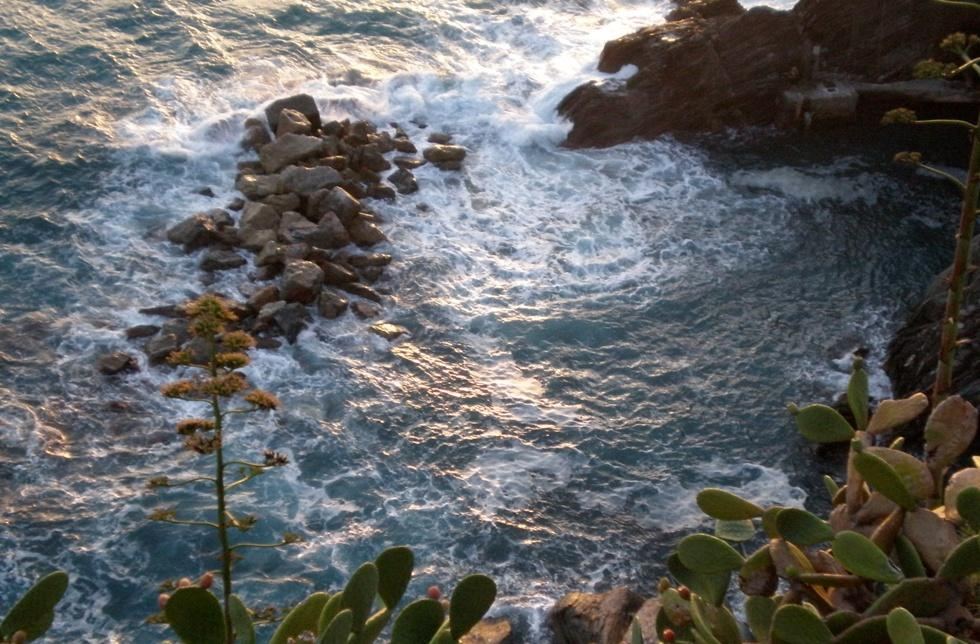
\includegraphics[width=0.415\textwidth]{./images/single_puzzle/pomeranz_805_14.jpg}}
	  &
	  \fbox{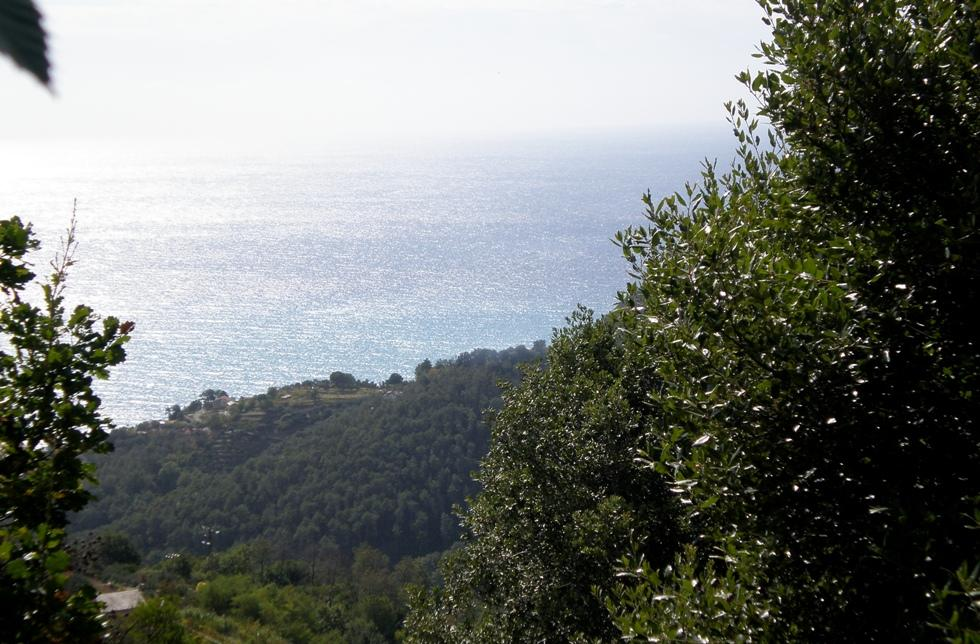
\includegraphics[width=0.415\textwidth]{./images/single_puzzle/pomeranz_805_12.jpg}}  
	  \\~\\	
	  \small Perfectly Reconstructed Image~(a)
	  & 
	  \small Misclassified Image~(b)
  \end{tabular}
\end{frame}
%%%%%%%%%%%%%%%%



\begin{frame}{Determining Input Puzzle Count}{Multiple Input Puzzles}
  \begin{itemize}
    \onslide<1->{
      \item \textbf{Goal}: Measure the Mixed-Bag Solver's accuracy determining the input puzzle count for multiple images
      \vfill
      \item \textbf{Procedure}: Randomly select a specified number of images (between 2 and 5) from the 20 image data set.
    }
    \vfill    
    \onslide<2->{      
      \item \textbf{Input Puzzle Count Error}: Difference between the actual number of input puzzles and the number determined by the Mixed-Bag Solver.
      \begin{itemize}
        \vspace{0.4em}
        \item \textbf{Example}: If 3 images were supplied to the solver but it determined there were 4, the error would be 1.
      \end{itemize}
    }
  \end{itemize}
\end{frame}
%%%%%%%%%%%%%%%%



\begin{frame}{Determining Input Puzzle Count}{Multiple Input Puzzles -- Results}
   \onslide<1->{
     \begin{center}
       \begin{scaletikzpicturetowidth}{0.9\textwidth}
        \begin{tikzpicture}[scale=\tikzscale]
          \begin{axis}[
                ybar, axis on top,
                height=8cm, width=12cm,
            	axis background/.style={fill=gray!10},
                bar width=0.4cm,
                ymajorgrids, tick align=inside,
                major grid style={draw=white},
                enlarge y limits={value=.1,upper},
                ymin=0, ymax=100,
                axis x line*=bottom,
                axis y line*=left,
                y axis line style={opacity=1},
                tickwidth=0pt,
                title=\textbf{Mixed-Bag Solver's Input Puzzle Count Error Frequency},
                enlarge x limits=0.2,
                legend style={
                    at={(0.5,-0.2)},
                    anchor=north,
                    legend columns=-1,
                    /tikz/every even column/.append style={column sep=0.5cm}
                },
                xlabel={Size of Input Puzzle Count Error},
                ylabel={Frequency (\%)},
                symbolic x coords={
                   0, 1, 2, 3},
               xtick=data,
               nodes near coords={
                \pgfmathprintnumber[precision=0]{\pgfplotspointmeta}
               }
            ]
        \addplot [fill=blue!30]
            coordinates {(0,74.5) (1,16.4) (2,7.3) (3,1.8)};
        \addplot [fill=red!30]
            coordinates {(0,44) (1,48) (2,4) (3,4)};
        \addplot [fill=green!30]
            coordinates {(0,50) (1,50) (2,0) (3,0)};
        \addplot [fill=gray]
            coordinates {(0,60) (1,20) (2,20) (3,0)};
        \legend{2 Puzzles, 3 Puzzles, 4 Puzzles, 5 Puzzles}
        \end{axis}
        \end{tikzpicture}
      \end{scaletikzpicturetowidth}  
    \end{center}
  }
\end{frame}
%%%%%%%%%%%%%%%%




\begin{frame}{Determining Input Puzzle Count}{Multiple Input Puzzles -- Results Summary}
  \begin{itemize}
    \onslide<1->{
      \item \textbf{Overall Accuracy}: 65\%
      \vfill
      \item \textbf{Iterations with Error Greater than One}: 8\%
      \vfill
      \item Accuracy did not significantly degrade as the number of input puzzles increased.
      \vfill
    }
    \onslide<2->{      
      \item \textbf{Over-Rejection of Cluster Mergers}: The Mixed-Bag Solver never underestimated the number of input puzzles.
      \begin{itemize}
        \vspace{0.4em}
        \item Performance may be improved by reducing the minimum clustering similarity threshold or minimum segment size
      \end{itemize}
    }
  \end{itemize}
\end{frame}
%%%%%%%%%%%%%%%%



\subsection{Solver Comparison}
\begin{frame}{Experimental Results}{Performance on Multiple Input Puzzles}

  \begin{itemize}
    \onslide<1->{
      \item \textbf{Goal}: Compare the performance of the Mixed-Bag Solver ({\color{spartanBlue}\textbf{MBS}}) and Paikin~\& Tal's algorithm 
      \vfill
      \item \textbf{Procedure:} Randomly select a specified number of images and input them into both solvers.
      \vfill
      \item \textbf{Quality Metrics Used}:
      \begin{itemize}
        \item Shiftable Enhanced Direct Accuracy Score (SEDAS)
        \item Enhanced Neighbor Accuracy Score (ENAS)
        \item Perfect Reconstruction Percentage
      \end{itemize}
    }
    \vfill
    \onslide<2->{
      \item \textbf{Note}: The results include the Mixed-Bag Solver's performance when it correctly estimated the puzzle count.
      \begin{itemize}
        \vspace{0.4em}
        \item This represents the performance ceiling for optimal hierarchical clustering.
      \end{itemize}
    }
  \end{itemize}

\end{frame}
%%%%%%%%%%%%%%%%



\begin{frame}{Performance on Multiple Input Puzzles}{Shiftable Enhanced Direct Accuracy Score (SEDAS)}
     \begin{center}
       \begin{scaletikzpicturetowidth}{0.9\textwidth}
        \begin{tikzpicture}[scale=\tikzscale]
          \begin{axis}[
            height=8cm, width=12cm,
            axis background/.style={fill=gray!10},
            title=\textbf{Effect of the Number of Input Puzzles on SEDAS},
            xlabel={\textbf{Number of Input Puzzles}},
            ylabel={\textbf{SEDAS}},
            xmin=1.5, xmax=5.5,
            ymin=0, ymax=1,
            xtick={2, 3, 4, 5},
            ytick={0,0.2,0.4,0.6,0.8,1.0},
            ymajorgrids=true,
            grid style=dashed,
            legend style={ at={(0.5,-0.25)}, anchor=north, legend columns=-1, /tikz/every even column/.append style={column sep=0.5cm}}
            ]
        \addplot [color=blue,mark=*,mark options={fill=blue},ultra thick]
            coordinates {(2,0.849835) (3,0.953583)
                 (4,0.88068) (5,0.792796)};
        \addplot [color=red,mark=square*,mark options={fill=red},ultra thick]
            coordinates {(2,0.757159) (3,0.799822)
                 (4,0.777987) (5,0.782815)};
        \addplot [color=darkGreen,mark=triangle*,mark options={fill=darkGreen},ultra thick]
            coordinates {(2,0.321232) (3,0.202879)
                 (4,0.108857) (5,0.09866)};
        \legend{MBS Correct Puzzle Count, MBS All, Paikin \& Tal}
        \end{axis}
        \end{tikzpicture}
      \end{scaletikzpicturetowidth}  
    \end{center}
\end{frame}
%%%%%%%%%%%%%%%%



\begin{frame}{Performance on Multiple Input Puzzles}{Enhanced Neighbor Accuracy Score (ENAS)}
     \begin{center}
       \begin{scaletikzpicturetowidth}{0.9\textwidth}
        \begin{tikzpicture}[scale=\tikzscale]
          \begin{axis}[
            height=8cm, width=12cm,
            axis background/.style={fill=gray!10},
            title=\textbf{Effect of the Number of Input Puzzles on ENAS},
            xlabel={\textbf{Number of Input Puzzles}},
            ylabel={\textbf{ENAS}},
            xmin=1.5, xmax=5.5,
            ymin=0, ymax=1,
            xtick={2, 3, 4, 5},
            ytick={0,0.2,0.4,0.6,0.8,1.0},
            ymajorgrids=true,
            grid style=dashed,
            legend style={ at={(0.5,-0.25)}, anchor=north, legend columns=-1, /tikz/every even column/.append style={column sep=0.5cm}}
            ]
			\addplot [color=blue,mark=*,mark options={fill=blue},ultra thick]
	coordinates {(2,0.932805) (3,0.955051)
		 (4,0.919987) (5,0.868454)};
			\addplot [color=red,mark=square*,mark options={fill=red},ultra thick]
	coordinates {(2,0.874472) (3,0.868832)
		 (4,0.862183) (5,0.876654)};
			\addplot [color=darkGreen,mark=triangle*,mark options={fill=darkGreen},ultra thick]
	coordinates {(2,0.462006) (3,0.364242)
		 (4,0.259996) (5,0.204337)};
        \legend{MBS Correct Puzzle Count, MBS All, Paikin \& Tal}
        \end{axis}
        \end{tikzpicture}
      \end{scaletikzpicturetowidth}  
    \end{center}
\end{frame}
%%%%%%%%%%%%%%%%




\begin{frame}{Performance on Multiple Input Puzzles}{Perfect Reconstruction Percentage}
     \begin{center}
       \begin{scaletikzpicturetowidth}{0.9\textwidth}
        \begin{tikzpicture}[scale=\tikzscale]
          \begin{axis}[
            height=8cm, width=12cm,
            axis background/.style={fill=gray!10},
            title=\textbf{Effect of the Number of Input Puzzles on ENAS},
            xlabel={\textbf{Number of Input Puzzles}},
            ylabel={\textbf{Perfect Reconstruction (\%)}},
            xmin=1.5, xmax=5.5,
            ymin=0, ymax=30,
            xtick={2, 3, 4, 5},
            ytick={0,5,10,15,20,25,30},
            ymajorgrids=true,
            grid style=dashed,
            legend style={ at={(0.5,-0.25)}, anchor=north, legend columns=-1, /tikz/every even column/.append style={column sep=0.5cm}}
            ]
			\addplot [color=blue,mark=*,mark options={fill=blue},ultra thick]
	coordinates {(2,29.3) (3,18.5)
		 (4,25.0) (5,20.0)};
			\addplot [color=red,mark=square*,mark options={fill=red},ultra thick]
	coordinates {(2,23.6) (3,18.8)
		 (4,15.6) (5,24.0)};
			\addplot [color=darkGreen,mark=triangle*,mark options={fill=darkGreen},ultra thick]
	coordinates {(2,5.5) (3,1.4)
		 (4,0) (5,0)};
        \legend{MBS Correct Puzzle Count, MBS All, Paikin \& Tal}
        \end{axis}
        \end{tikzpicture}
      \end{scaletikzpicturetowidth}  
    \end{center}
\end{frame}
%%%%%%%%%%%%%%%%



\begin{frame}{Performance on Multiple Input Puzzles}{Results Summary}
  \begin{itemize}
    \onslide<1->{
      \item \textbf{Summary}: The Mixed-Bag Solver significantly outperformed Paikin~\& Tal's algorithm across all metrics. 
      \vspace{0.4em} 
      \begin{itemize}
        \item This is notwithstanding that only their algorithm was supplied with the number of input puzzles.
      \end{itemize}
    }
    \vfill
    \onslide<2->{
      \item \textbf{Puzzle Input Count}: Unlike Paikin~\& Tal's algorithm, the Mixed-Bag Solver saw no significant decrease in performance with additional input puzzles
    }
    \vfill
    \onslide<3->{
      \item \textbf{Effect of Clustering Errors}: Performance only decreased slightly when incorrectly estimated input puzzle count.
      \vspace{0.4em} 
      \begin{itemize}
        \item Many of the extra puzzles were relatively insignificant in size
      \end{itemize}
    }
  \end{itemize}
\end{frame}
%%%%%%%%%%%%%%%%




\section{Conclusions}
\transitionFrame{Conclusions}



\begin{frame}{Conclusions}{}
  \onslide<2->{
    \begin{itemize}
      \setlength\itemsep{1em}
      \item This thesis presented a fully-automated solver for Mixed-Bag puzzles.
      \vfill
      \item Mixed-Bag Solver significantly outperforms the current state of the art while receiving no externally supplied information.
      \vfill
      \item Introduced the first set of solver quality metrics for Mixed-Bag puzzles.
    \end{itemize}  
  }
\end{frame}
%%%%%%%%%%%%%%%%



%%%%%%%%%%%%%%%%%%%%%%%%%%%%%%%%%%%%%%%%%%%%%%%%%%%%%%%%%%%%%%%%%%%%
%%%%%%               APPENDIX / BACK-UP SLIDES                %%%%%%
%%%%%%%%%%%%%%%%%%%%%%%%%%%%%%%%%%%%%%%%%%%%%%%%%%%%%%%%%%%%%%%%%%%%

% Stop numbering the slides
\backupbegin

% Add an appendix slide to break up the flow
\appendix

\section*{}  % Close the previous section

\section{Conclusions}
\subsection{Future Work}
\begin{frame}{Conclusions}{Future Work}
  \begin{itemize}
    \setlength\itemsep{.8em}
    \item<1-> Improved Assembler
    \begin{itemize}
      \setlength\itemsep{.8em}
    	\item<1-> Prioritize placement using multiple best buddies
    	\item<1-> Address placement performance in regions with low best buddy density
    \end{itemize}
    \vfill
    \item<2-> Dynamic determination of the segment clustering threshold
    \vfill
    \item<3-> Expanded stitching piece selection
  \end{itemize}
\end{frame}
%%%%%%%%%%%%%%%%

% Add the list of references
\begin{frame}[t,allowframebreaks]{List of References}
	\bibliographystyle{ieeetr}
	{\tiny \bibliography{references}}
\end{frame}


\section{Introduction}
\subsection{Puzzle Types}
\begin{frame}{Introduction}{Jig Swap Puzzle Types}
\onslide<1->{There are four primary jig swap puzzle types as formalized by~\cite{gallagher2012}. In all cases, the ``ground-truth'' input is unknown.} 
    \vfill
    \begin{itemize}
        \item<2-> \textbf{Type~1}: Puzzle dimensions and piece rotation are known.  May have ``anchor'' piece(s) fixed in the correct location(s).
        \vfill
        \item<3-> \textbf{Type~2}: All piece locations and rotations unknown.  Puzzle dimensions may be known.
        \vfill
        \item<4-> \textbf{Type~3}: All piece locations are known.  Only rotation is unknown.
        \vfill
        \item<5-> \textbf{Mixed-Bag}: Pieces come from multiple puzzles
    \end{itemize}
    \vfill
    \onslide<6->{Mixed-Bag puzzles are the focus of this thesis.}
\end{frame}
%%%%%%%%%%%%%%%%

\subsection{Previous Work}
\begin{frame}{Previous Work}{}
    \begin{itemize}
        \onslide<1->{\item \textbf{Cho \textit{et al.}}~\cite{cho2010} -- Introduced the first modern jig swap puzzle solver
        \vspace{0.4em}
        \begin{itemize}
            \setlength\itemsep{0.6em}
            \item Graphical model-based Type~1 solver
            \item Puzzle dimensions are known
            \item Used one or more anchor pieces
            \item Defined quality metrics for Type~1 and Type~2 puzzles
            \item Established the standard comparative test conditions
        \end{itemize}}
        \vfill
        \onslide<2->{\item \textbf{Pomeranz \textit{et al.}}~\cite{pomeranz2011} -- Iterative, greedy Type~1 puzzle solver
        \begin{itemize}
            \setlength\itemsep{.6em}
            \item Eliminated the use of anchor pieces 
            \item Created multiple solver benchmarks of various sizes
        \end{itemize}}
    \end{itemize}
\end{frame}
%%%%%%%%%%%%%%%%



\section{Best Buddies}
\begin{frame}{Introduction}{Best Buddies}\label{frame:bestBuddies}
    \begin{itemize}
        \item \textbf{Basis of all Modern Jig Swap Solvers}: The more compatible two pieces are, the more likely they are to be adjacent.
        \vfill
        \item \textbf{Best Buddies}: A pair of puzzles pieces that are more compatible with each other on their respective sides than they are to any other piece~\cite{pomeranz2011}
        \begin{itemize}
          \item \textbf{Note}: Not all puzzle pieces will have a best buddy.
        \end{itemize}
        \vfill
				\begin{equation}\label{eq:pomeranzBestBuddyDefinition}
					\centering
					\begin{split}
						\begin{matrix}
								\forall{p_{k}}\forall{s_z},C(p_i, s_x, p_j, s_y) \geq C(p_i, s_x, p_k, s_z)
								\\
								\\
								\textnormal{and}
								\\
								\\
								\forall{p_{k}}\forall{s_z},C(p_j, s_y, p_i, s_x) \geq C(p_j, s_y, p_k, s_z)
						\end{matrix}
					\end{split}
				\end{equation} 
        \vfill
        \item \textbf{Importance of Best Buddies}: Key adjacency indicator
    \end{itemize}
\end{frame}
%%%%%%%%%%%%%%%%



\subsection{Best Buddy Density}
\begin{frame}{Quantifying Solver Quality}{Best Buddy Density}
  \begin{itemize}
    \setlength\itemsep{1em}
    \item \textbf{Best Buddy Density} (BBD): A metric for quantifying the best buddy profile of an image that is independent of image size.
  \end{itemize}
  \vfill
  \begin{equation} \label{eq:bestBuddyDensity}
    BBD = \frac{b}{n \cdot q}
  \end{equation}
  \vspace{-0.6em}
  \begin{itemize}
    \vfill
    \item A greater BBD means the pieces are more differentiated making the puzzle easier to solve.
  \end{itemize}
\end{frame}
%%%%%%%%%%%%%%%%


\begin{frame}{Best Buddy Density}{Visualization}  
  \begin{block}{\textbf{Visualizing Best Buddy Density}}
    \begin{itemize}
      \setlength\itemsep{1em}
      \item Transform each puzzle piece into a square consisting of four isosceles triangles.
      \item Color each triangle according to whether the adjacent piece is a best buddy.  The scheme used in this thesis:
    \end{itemize}
    {\footnotesize 
	    {\setlength\extrarowheight{2pt}
		    \begin{table}
		      \begin{center}
		        \begin{tabular}{ | >{\centering\arraybackslash}m{0.62in} | >{\centering\arraybackslash}m{0.78in} | >{\centering\arraybackslash}m{0.7in} | >{\centering\arraybackslash}m{0.62in} | }
		          \Xhline{1pt}
			        \textbf{No Best Buddy} 
			        & \textbf{Non-Adjacent Best Buddy}
			        & \textbf{Adjacent Best Buddy}
			        & \textbf{No Piece Present}
			        \\ \hline \hline
		          {\tiny \cellcolor{white}~} 
		          & {\tiny \cellcolor{red}~} 
		          & {\tiny \cellcolor{green}~} 
		          & {\tiny \cellcolor{black}~} 
		          \\
		          {\tiny \cellcolor{white}~} 
		          & {\tiny \cellcolor{red}~} 
		          & {\tiny \cellcolor{green}~} 
		          & {\tiny \cellcolor{black}~}
		          \\ \Xhline{1pt}
		        \end{tabular}
		      \end{center}
		    \end{table}
		  }}
    \begin{itemize}
      \setlength\itemsep{1em}
      \item Areas with higher best buddy density will have more green triangles.
    \end{itemize}
  \end{block}
\end{frame}
%%%%%%%%%%%%%%%%


\begin{frame}{Best Buddy Density}{Visualization Example}  

{\small
	\begin{figure}[t]
	  \centering
	  \begin{tabular}{ >{\centering\arraybackslash}m{0.40\textwidth} >{\centering\arraybackslash}m{0.40\textwidth} }
	     \onslide<1->{\fbox{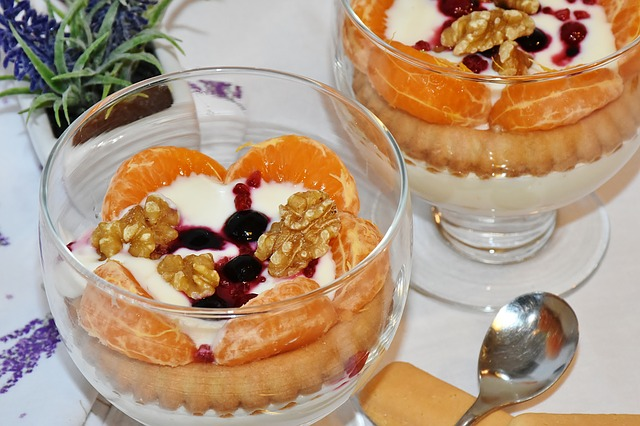
\includegraphics[width=0.37\textwidth]{./images/dessert_pixabay.jpg}}}  
	     & \onslide<2->{\fbox{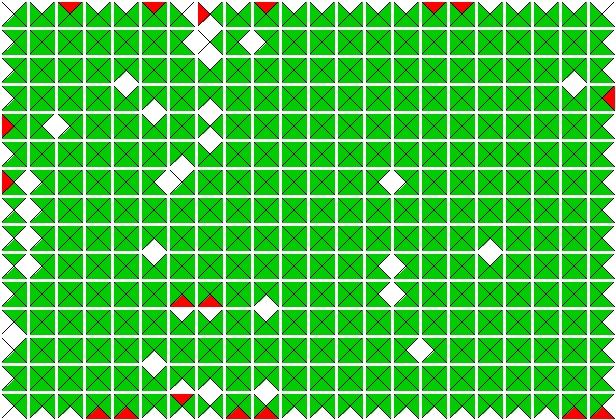
\includegraphics[width=0.37\textwidth]{./images/dessert_best_buddy_visualization.jpg}}}
	     \\~\\
	     \onslide<1->{Original Image~\cite{pixabay}} 
	     & \onslide<2->{Best Buddy Visualization}
	  \end{tabular}
	\label{fig:bestBuddyVisualization}
	\end{figure}
}

\end{frame}
%%%%%%%%%%%%%%%%



\section{Experimental Results}

\subsection{Single Input Puzzle}
\begin{frame}{Determining Input Puzzle Count}{Comparison of Best Buddy Density for Misclassified Images}
  \begin{tabular}{ >{\centering\arraybackslash}m{0.45\textwidth} >{\centering\arraybackslash}m{0.45\textwidth} }

	  \onslide<1->{
	    \fbox{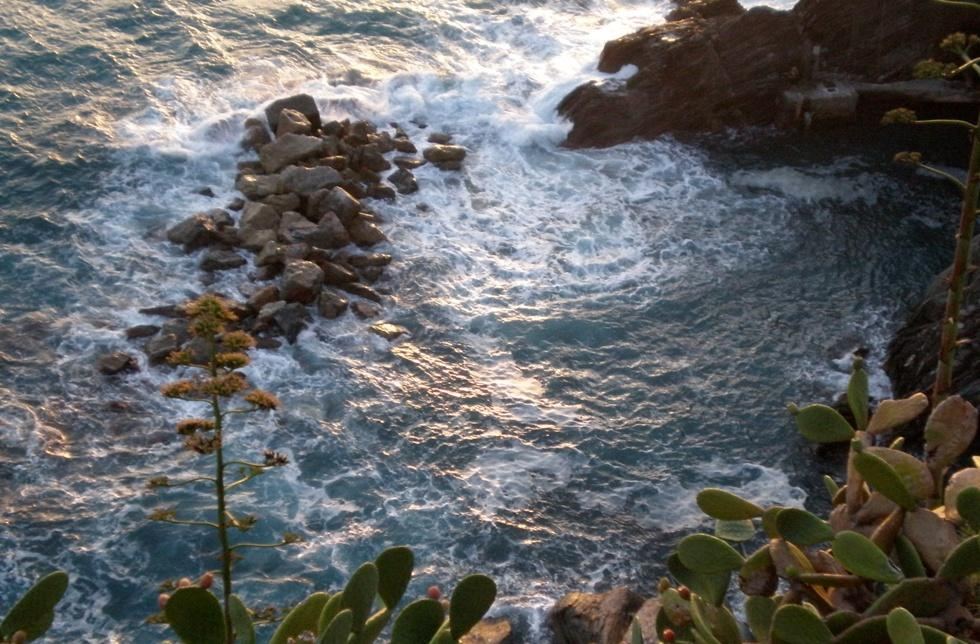
\includegraphics[width=0.35\textwidth]{./images/single_puzzle/pomeranz_805_14.jpg}}
	  } & 
	  \onslide<2->{
	    \fbox{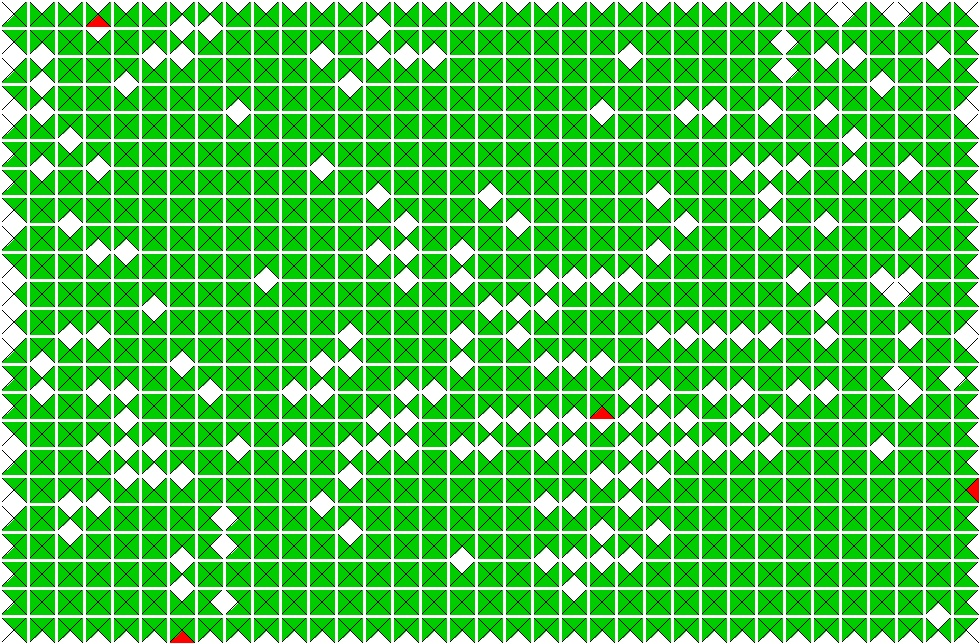
\includegraphics[width=0.35\textwidth]{./images/single_puzzle/best_buddies_pomeranz_805_14.jpg}}
	  } 	    
	  \\~\\	
	  \onslide<1->{
	    \small Perfectly Reconstructed Image~(a)
	  } & 
	  \onslide<2->{\small Best Buddy Visualization~(a) 
	  }	  
    \\~\\	  
	  \onslide<1->{
	    \fbox{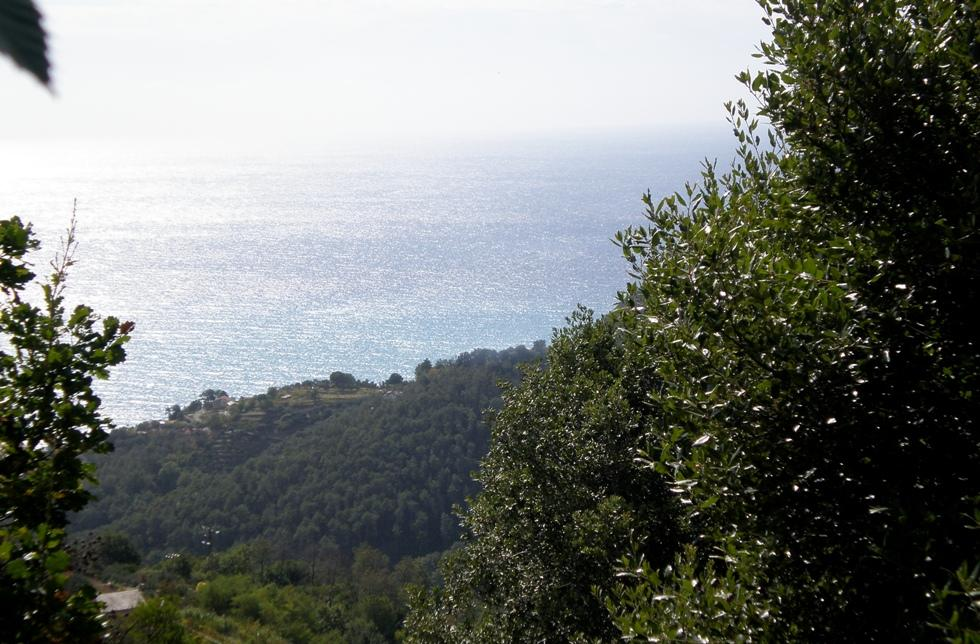
\includegraphics[width=0.35\textwidth]{./images/single_puzzle/pomeranz_805_12.jpg}}
	  } & 
	  \onslide<2->{
	    \fbox{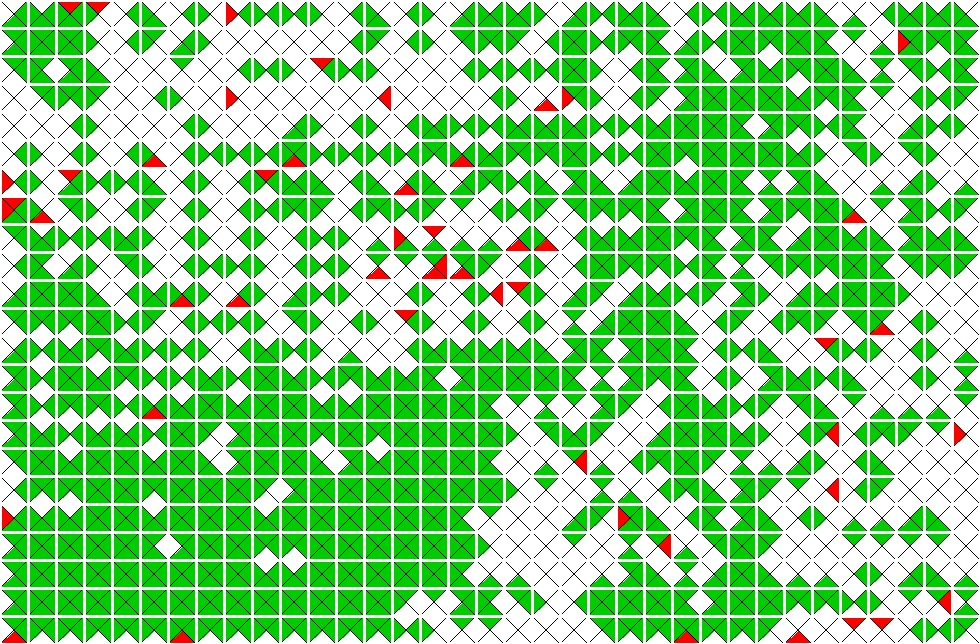
\includegraphics[width=0.35\textwidth]{./images/single_puzzle/best_buddies_pomeranz_805_12.jpg}}
	  } 
	  \\~\\
	  \onslide<1->{
	    \small Misclassified Image~(b)
	  } & 
	  \onslide<2->{
	    \small Best Buddy Visualization~(b)
	  }
  \end{tabular}
\end{frame}
%%%%%%%%%%%%%%%%


\subsection{Ten Puzzle Results}
\begin{frame}{Experimental Results}{Solving More than Five Puzzles}
  \begin{itemize}
	  \item<1-> As the number of puzzles increases, the difficulty of simultaneously reconstructing them also increases.
	  \vfill  
  	\item<2-> \textbf{Current State of the Art}: Paikin~\& Tal~\cite{paikin2015} solved up to five puzzles simultaneously.
	  \vfill
  	\item<3-> \textbf{Goal}: Compare the performance of the Mixed-Bag Solver and Paikin~\& Tal's algorithm on 10~puzzles.
  \end{itemize}
\end{frame}
%%%%%%%%%%%%%%%%


\begin{frame}{Ten Puzzle Results}{Summary}
  	\begin{itemize}
  		\item<1-> \textbf{Paikin~\& Tal}
  	  \vspace{0.4em}
  		\begin{itemize}
  		  \setlength\itemsep{0.7em}
			  \item Seed of nine images came from just three input images
			  \item SEDAS and EDAS greater than 0.9 for only one image
			  \item No perfectly reconstructed images
		  \end{itemize}
		  \vfill
  	  \item<2-> \textbf{Mixed-Bag Solver}
  	  \vspace{0.4em}
		  \begin{itemize}
		    \setlength\itemsep{0.7em}
			  \item SEDAS and EDAS greater than 0.9 for all images
			  \item Four images perfectly reconstructed
			  \item Results comparable to Paikin~\& Tal's algorithm solving each puzzle individually
		  \end{itemize}	
  \end{itemize}
\end{frame}
%%%%%%%%%%%%%%%%





\backupend



\end{document}
